\documentclass[twoside]{book}

% Packages required by doxygen
\usepackage{fixltx2e}
\usepackage{calc}
\usepackage{doxygen}
\usepackage[export]{adjustbox} % also loads graphicx
\usepackage{graphicx}
\usepackage[utf8]{inputenc}
\usepackage{makeidx}
\usepackage{multicol}
\usepackage{multirow}
\PassOptionsToPackage{warn}{textcomp}
\usepackage{textcomp}
\usepackage[nointegrals]{wasysym}
\usepackage[table]{xcolor}

% Font selection
\usepackage[T1]{fontenc}
\usepackage[scaled=.90]{helvet}
\usepackage{courier}
\usepackage{amssymb}
\usepackage{sectsty}
\renewcommand{\familydefault}{\sfdefault}
\allsectionsfont{%
  \fontseries{bc}\selectfont%
  \color{darkgray}%
}
\renewcommand{\DoxyLabelFont}{%
  \fontseries{bc}\selectfont%
  \color{darkgray}%
}
\newcommand{\+}{\discretionary{\mbox{\scriptsize$\hookleftarrow$}}{}{}}

% Page & text layout
\usepackage{geometry}
\geometry{%
  a4paper,%
  top=2.5cm,%
  bottom=2.5cm,%
  left=2.5cm,%
  right=2.5cm%
}
\tolerance=750
\hfuzz=15pt
\hbadness=750
\setlength{\emergencystretch}{15pt}
\setlength{\parindent}{0cm}
\setlength{\parskip}{3ex plus 2ex minus 2ex}
\makeatletter
\renewcommand{\paragraph}{%
  \@startsection{paragraph}{4}{0ex}{-1.0ex}{1.0ex}{%
    \normalfont\normalsize\bfseries\SS@parafont%
  }%
}
\renewcommand{\subparagraph}{%
  \@startsection{subparagraph}{5}{0ex}{-1.0ex}{1.0ex}{%
    \normalfont\normalsize\bfseries\SS@subparafont%
  }%
}
\makeatother

% Headers & footers
\usepackage{fancyhdr}
\pagestyle{fancyplain}
\fancyhead[LE]{\fancyplain{}{\bfseries\thepage}}
\fancyhead[CE]{\fancyplain{}{}}
\fancyhead[RE]{\fancyplain{}{\bfseries\leftmark}}
\fancyhead[LO]{\fancyplain{}{\bfseries\rightmark}}
\fancyhead[CO]{\fancyplain{}{}}
\fancyhead[RO]{\fancyplain{}{\bfseries\thepage}}
\fancyfoot[LE]{\fancyplain{}{}}
\fancyfoot[CE]{\fancyplain{}{}}
\fancyfoot[RE]{\fancyplain{}{\bfseries\scriptsize Generated by Doxygen }}
\fancyfoot[LO]{\fancyplain{}{\bfseries\scriptsize Generated by Doxygen }}
\fancyfoot[CO]{\fancyplain{}{}}
\fancyfoot[RO]{\fancyplain{}{}}
\renewcommand{\footrulewidth}{0.4pt}
\renewcommand{\chaptermark}[1]{%
  \markboth{#1}{}%
}
\renewcommand{\sectionmark}[1]{%
  \markright{\thesection\ #1}%
}

% Indices & bibliography
\usepackage{natbib}
\usepackage[titles]{tocloft}
\setcounter{tocdepth}{3}
\setcounter{secnumdepth}{5}
\makeindex

% Hyperlinks (required, but should be loaded last)
\usepackage{ifpdf}
\ifpdf
  \usepackage[pdftex,pagebackref=true]{hyperref}
\else
  \usepackage[ps2pdf,pagebackref=true]{hyperref}
\fi
\hypersetup{%
  colorlinks=true,%
  linkcolor=blue,%
  citecolor=blue,%
  unicode%
}

% Custom commands
\newcommand{\clearemptydoublepage}{%
  \newpage{\pagestyle{empty}\cleardoublepage}%
}

\usepackage{caption}
\captionsetup{labelsep=space,justification=centering,font={bf},singlelinecheck=off,skip=4pt,position=top}

%===== C O N T E N T S =====

\begin{document}

% Titlepage & ToC
\hypersetup{pageanchor=false,
             bookmarksnumbered=true,
             pdfencoding=unicode
            }
\pagenumbering{alph}
\begin{titlepage}
\vspace*{7cm}
\begin{center}%
{\Large Arkav\+Quarium }\\
\vspace*{1cm}
{\large Generated by Doxygen 1.8.15}\\
\end{center}
\end{titlepage}
\clearemptydoublepage
\pagenumbering{roman}
\tableofcontents
\clearemptydoublepage
\pagenumbering{arabic}
\hypersetup{pageanchor=true}

%--- Begin generated contents ---
\chapter{Hierarchical Index}
\section{Class Hierarchy}
This inheritance list is sorted roughly, but not completely, alphabetically\+:\begin{DoxyCompactList}
\item \contentsline{section}{Aquarium\+Object}{\pageref{class_aquarium_object}}{}
\begin{DoxyCompactList}
\item \contentsline{section}{Coin}{\pageref{class_coin}}{}
\item \contentsline{section}{Fish\+Food}{\pageref{class_fish_food}}{}
\item \contentsline{section}{Guppy}{\pageref{class_guppy}}{}
\item \contentsline{section}{Piranha}{\pageref{class_piranha}}{}
\item \contentsline{section}{Snail}{\pageref{class_snail}}{}
\end{DoxyCompactList}
\item \contentsline{section}{Fish}{\pageref{interface_fish}}{}
\begin{DoxyCompactList}
\item \contentsline{section}{Guppy}{\pageref{class_guppy}}{}
\item \contentsline{section}{Piranha}{\pageref{class_piranha}}{}
\end{DoxyCompactList}
\item \contentsline{section}{Linked\+List$<$ T $>$}{\pageref{class_linked_list}}{}
\item \contentsline{section}{Linked\+List$<$ Coin $>$}{\pageref{class_linked_list}}{}
\item \contentsline{section}{Linked\+List$<$ Fish\+Food $>$}{\pageref{class_linked_list}}{}
\item \contentsline{section}{Linked\+List$<$ Guppy $>$}{\pageref{class_linked_list}}{}
\item \contentsline{section}{Linked\+List$<$ Piranha $>$}{\pageref{class_linked_list}}{}
\item \contentsline{section}{Main}{\pageref{class_main}}{}
\item \contentsline{section}{Node$<$ T $>$}{\pageref{class_node}}{}
\item \contentsline{section}{Node$<$ Integer $>$}{\pageref{class_node}}{}
\item J\+Panel\begin{DoxyCompactList}
\item \contentsline{section}{Aquarium}{\pageref{class_aquarium}}{}
\end{DoxyCompactList}
\item Mouse\+Listener\begin{DoxyCompactList}
\item \contentsline{section}{Aquarium}{\pageref{class_aquarium}}{}
\end{DoxyCompactList}
\end{DoxyCompactList}

\chapter{Class Index}
\section{Class List}
Here are the classes, structs, unions and interfaces with brief descriptions\+:\begin{DoxyCompactList}
\item\contentsline{section}{\mbox{\hyperlink{class_aquarium}{Aquarium}} }{\pageref{class_aquarium}}{}
\item\contentsline{section}{\mbox{\hyperlink{class_aquarium_object}{Aquarium\+Object}} }{\pageref{class_aquarium_object}}{}
\item\contentsline{section}{\mbox{\hyperlink{class_coin}{Coin}} }{\pageref{class_coin}}{}
\item\contentsline{section}{\mbox{\hyperlink{interface_fish}{Fish}} }{\pageref{interface_fish}}{}
\item\contentsline{section}{\mbox{\hyperlink{class_fish_food}{Fish\+Food}} }{\pageref{class_fish_food}}{}
\item\contentsline{section}{\mbox{\hyperlink{class_guppy}{Guppy}} }{\pageref{class_guppy}}{}
\item\contentsline{section}{\mbox{\hyperlink{class_linked_list}{Linked\+List$<$ T $>$}} }{\pageref{class_linked_list}}{}
\item\contentsline{section}{\mbox{\hyperlink{class_main}{Main}} }{\pageref{class_main}}{}
\item\contentsline{section}{\mbox{\hyperlink{class_node}{Node$<$ T $>$}} }{\pageref{class_node}}{}
\item\contentsline{section}{\mbox{\hyperlink{class_piranha}{Piranha}} }{\pageref{class_piranha}}{}
\item\contentsline{section}{\mbox{\hyperlink{class_snail}{Snail}} }{\pageref{class_snail}}{}
\end{DoxyCompactList}

\chapter{Class Documentation}
\hypertarget{class_aquarium}{}\section{Aquarium Class Reference}
\label{class_aquarium}\index{Aquarium@{Aquarium}}


Inheritance diagram for Aquarium\+:
\nopagebreak
\begin{figure}[H]
\begin{center}
\leavevmode
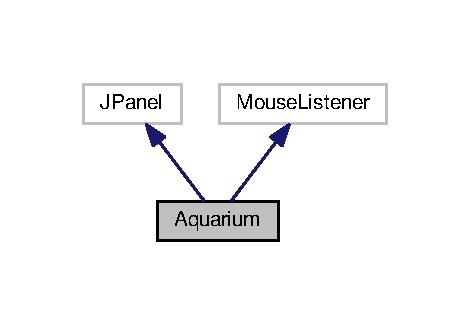
\includegraphics[width=226pt]{class_aquarium__inherit__graph}
\end{center}
\end{figure}


Collaboration diagram for Aquarium\+:
\nopagebreak
\begin{figure}[H]
\begin{center}
\leavevmode
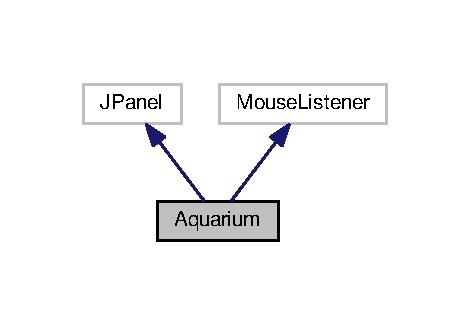
\includegraphics[width=226pt]{class_aquarium__coll__graph}
\end{center}
\end{figure}
\subsection*{Public Member Functions}
\begin{DoxyCompactItemize}
\item 
\mbox{\hyperlink{class_aquarium_a173f8b85de9d2f61c02d13ebdc05026c}{Aquarium}} ()
\item 
void \mbox{\hyperlink{class_aquarium_a534d2ac777989cb7b69167ca19d3c89e}{setx\+Click}} (final int p\+X\+Click)
\item 
void \mbox{\hyperlink{class_aquarium_a13fca2e9f118bbc3a150e22c72a5eeb7}{sety\+Click}} (final int p\+Y\+Click)
\item 
void \mbox{\hyperlink{class_aquarium_a2f943847eaa591471bd6d50dd17989f5}{set\+Egg\+State}} (final int p\+Egg\+State)
\item 
\mbox{\hyperlink{class_linked_list}{Linked\+List}}$<$ \mbox{\hyperlink{class_guppy}{Guppy}} $>$ \mbox{\hyperlink{class_aquarium_ac0ff36aa463290ad45aff4faf6889056}{get\+List\+Guppy}} ()
\item 
\mbox{\hyperlink{class_linked_list}{Linked\+List}}$<$ \mbox{\hyperlink{class_piranha}{Piranha}} $>$ \mbox{\hyperlink{class_aquarium_a168600416b33739a5943f44932325c29}{get\+List\+Piranha}} ()
\item 
\mbox{\hyperlink{class_linked_list}{Linked\+List}}$<$ \mbox{\hyperlink{class_coin}{Coin}} $>$ \mbox{\hyperlink{class_aquarium_ad7e90e4a2cd4a8810dfd497ba0f5375f}{get\+List\+Coin}} ()
\item 
\mbox{\hyperlink{class_linked_list}{Linked\+List}}$<$ \mbox{\hyperlink{class_fish_food}{Fish\+Food}} $>$ \mbox{\hyperlink{class_aquarium_a1bdc2bc59b49bd0c09aed6a51552d5f2}{get\+List\+Fish\+Food}} ()
\item 
\mbox{\hyperlink{class_snail}{Snail}} \mbox{\hyperlink{class_aquarium_ac00cb1b361c2b368370f3fd1225ff296}{get\+Snail}} ()
\item 
\mbox{\hyperlink{class_node}{Node}}$<$ Integer $>$ \mbox{\hyperlink{class_aquarium_aed777455bcb78b66ee3908b8be819372}{get\+Money}} ()
\item 
int \mbox{\hyperlink{class_aquarium_a081f2e1e4de0b98da501d2d067a3de0a}{get\+Egg\+State}} ()
\item 
void \mbox{\hyperlink{class_aquarium_a07837c9e2cd6167a3fbe4dfee5a1bda9}{mouse\+Clicked}} (final Mouse\+Event e)
\item 
void \mbox{\hyperlink{class_aquarium_a8f9a90754361531477cb8f13e2ebeeb4}{mouse\+Pressed}} (final Mouse\+Event e)
\item 
void \mbox{\hyperlink{class_aquarium_a9aa66d2632438550a97327f32f30e36d}{mouse\+Released}} (final Mouse\+Event e)
\item 
void \mbox{\hyperlink{class_aquarium_a5c7c79153603cb43ef13029f1a6f69a7}{mouse\+Entered}} (final Mouse\+Event e)
\item 
void \mbox{\hyperlink{class_aquarium_a7bb467907d03033dd70195526ae85b21}{mouse\+Exited}} (final Mouse\+Event e)
\item 
void \mbox{\hyperlink{class_aquarium_a5ea05fb764eeba71972deb3eb0fe6140}{paint}} (final Graphics g)
\end{DoxyCompactItemize}
\subsection*{Static Public Member Functions}
\begin{DoxyCompactItemize}
\item 
static void \mbox{\hyperlink{class_aquarium_a05ee79d2ed1f22d34a02ce301a2527c5}{set\+Egg\+Picture\+One}} (final Buffered\+Image p\+Egg\+Picture\+One)
\item 
static void \mbox{\hyperlink{class_aquarium_a7ff613dbc0b8c2ffdd7e0ce1b96a5d5f}{set\+Egg\+Picture\+Two}} (final Buffered\+Image p\+Egg\+Picture\+Two)
\item 
static void \mbox{\hyperlink{class_aquarium_a7f7c1d667dacf3e52f592ff20a939be0}{set\+Egg\+Picture\+Three}} (final Buffered\+Image p\+Egg\+Picture\+Three)
\item 
static void \mbox{\hyperlink{class_aquarium_ab59b9af7bb093e555e2b683dcf39e498}{set\+Background}} (final Buffered\+Image p\+Background)
\item 
static void \mbox{\hyperlink{class_aquarium_a4133a27a6feca8d8cdffaad0ada7da0f}{set\+Win\+Background}} (final Buffered\+Image p\+Win\+Background)
\item 
static void \mbox{\hyperlink{class_aquarium_a339b7094b59172816c41e5284411893e}{set\+Lose\+Background}} (final Buffered\+Image p\+Lose\+Background)
\item 
static void \mbox{\hyperlink{class_aquarium_a97fa4960f66a18b449a122ef11abcb0b}{set\+Menu\+Background}} (final Buffered\+Image p\+Menu\+Background)
\item 
static void \mbox{\hyperlink{class_aquarium_a65f0247ca0458a289572ec8cd375e9f1}{set\+Font\+Type}} (final Font p\+Font\+Type)
\end{DoxyCompactItemize}


\subsection{Detailed Description}
\mbox{\hyperlink{class_aquarium}{Aquarium}} class. This class instantiates \mbox{\hyperlink{class_aquarium}{Aquarium}}. 

\subsection{Constructor \& Destructor Documentation}
\mbox{\Hypertarget{class_aquarium_a173f8b85de9d2f61c02d13ebdc05026c}\label{class_aquarium_a173f8b85de9d2f61c02d13ebdc05026c}} 
\index{Aquarium@{Aquarium}!Aquarium@{Aquarium}}
\index{Aquarium@{Aquarium}!Aquarium@{Aquarium}}
\subsubsection{\texorpdfstring{Aquarium()}{Aquarium()}}
{\footnotesize\ttfamily Aquarium.\+Aquarium (\begin{DoxyParamCaption}{ }\end{DoxyParamCaption})\hspace{0.3cm}{\ttfamily [inline]}}

Instantiates a new \mbox{\hyperlink{class_aquarium}{Aquarium}}. 

\subsection{Member Function Documentation}
\mbox{\Hypertarget{class_aquarium_a081f2e1e4de0b98da501d2d067a3de0a}\label{class_aquarium_a081f2e1e4de0b98da501d2d067a3de0a}} 
\index{Aquarium@{Aquarium}!get\+Egg\+State@{get\+Egg\+State}}
\index{get\+Egg\+State@{get\+Egg\+State}!Aquarium@{Aquarium}}
\subsubsection{\texorpdfstring{get\+Egg\+State()}{getEggState()}}
{\footnotesize\ttfamily int Aquarium.\+get\+Egg\+State (\begin{DoxyParamCaption}{ }\end{DoxyParamCaption})\hspace{0.3cm}{\ttfamily [inline]}}

Get egg state.

\begin{DoxyReturn}{Returns}
egg\+State 
\end{DoxyReturn}
\mbox{\Hypertarget{class_aquarium_ad7e90e4a2cd4a8810dfd497ba0f5375f}\label{class_aquarium_ad7e90e4a2cd4a8810dfd497ba0f5375f}} 
\index{Aquarium@{Aquarium}!get\+List\+Coin@{get\+List\+Coin}}
\index{get\+List\+Coin@{get\+List\+Coin}!Aquarium@{Aquarium}}
\subsubsection{\texorpdfstring{get\+List\+Coin()}{getListCoin()}}
{\footnotesize\ttfamily \mbox{\hyperlink{class_linked_list}{Linked\+List}}$<$\mbox{\hyperlink{class_coin}{Coin}}$>$ Aquarium.\+get\+List\+Coin (\begin{DoxyParamCaption}{ }\end{DoxyParamCaption})\hspace{0.3cm}{\ttfamily [inline]}}

Get list of \mbox{\hyperlink{class_coin}{Coin}}.

\begin{DoxyReturn}{Returns}
\mbox{\hyperlink{class_linked_list}{Linked\+List$<$\+Coin$>$}} 
\end{DoxyReturn}
\mbox{\Hypertarget{class_aquarium_a1bdc2bc59b49bd0c09aed6a51552d5f2}\label{class_aquarium_a1bdc2bc59b49bd0c09aed6a51552d5f2}} 
\index{Aquarium@{Aquarium}!get\+List\+Fish\+Food@{get\+List\+Fish\+Food}}
\index{get\+List\+Fish\+Food@{get\+List\+Fish\+Food}!Aquarium@{Aquarium}}
\subsubsection{\texorpdfstring{get\+List\+Fish\+Food()}{getListFishFood()}}
{\footnotesize\ttfamily \mbox{\hyperlink{class_linked_list}{Linked\+List}}$<$\mbox{\hyperlink{class_fish_food}{Fish\+Food}}$>$ Aquarium.\+get\+List\+Fish\+Food (\begin{DoxyParamCaption}{ }\end{DoxyParamCaption})\hspace{0.3cm}{\ttfamily [inline]}}

Get list of \mbox{\hyperlink{class_fish_food}{Fish\+Food}}.

\begin{DoxyReturn}{Returns}
\mbox{\hyperlink{class_linked_list}{Linked\+List$<$\+Fish\+Food$>$}} 
\end{DoxyReturn}
\mbox{\Hypertarget{class_aquarium_ac0ff36aa463290ad45aff4faf6889056}\label{class_aquarium_ac0ff36aa463290ad45aff4faf6889056}} 
\index{Aquarium@{Aquarium}!get\+List\+Guppy@{get\+List\+Guppy}}
\index{get\+List\+Guppy@{get\+List\+Guppy}!Aquarium@{Aquarium}}
\subsubsection{\texorpdfstring{get\+List\+Guppy()}{getListGuppy()}}
{\footnotesize\ttfamily \mbox{\hyperlink{class_linked_list}{Linked\+List}}$<$\mbox{\hyperlink{class_guppy}{Guppy}}$>$ Aquarium.\+get\+List\+Guppy (\begin{DoxyParamCaption}{ }\end{DoxyParamCaption})\hspace{0.3cm}{\ttfamily [inline]}}

Get list of \mbox{\hyperlink{class_guppy}{Guppy}}.

\begin{DoxyReturn}{Returns}
\mbox{\hyperlink{class_linked_list}{Linked\+List$<$\+Guppy$>$}} 
\end{DoxyReturn}
\mbox{\Hypertarget{class_aquarium_a168600416b33739a5943f44932325c29}\label{class_aquarium_a168600416b33739a5943f44932325c29}} 
\index{Aquarium@{Aquarium}!get\+List\+Piranha@{get\+List\+Piranha}}
\index{get\+List\+Piranha@{get\+List\+Piranha}!Aquarium@{Aquarium}}
\subsubsection{\texorpdfstring{get\+List\+Piranha()}{getListPiranha()}}
{\footnotesize\ttfamily \mbox{\hyperlink{class_linked_list}{Linked\+List}}$<$\mbox{\hyperlink{class_piranha}{Piranha}}$>$ Aquarium.\+get\+List\+Piranha (\begin{DoxyParamCaption}{ }\end{DoxyParamCaption})\hspace{0.3cm}{\ttfamily [inline]}}

Get list of \mbox{\hyperlink{class_piranha}{Piranha}}.

\begin{DoxyReturn}{Returns}
\mbox{\hyperlink{class_linked_list}{Linked\+List$<$\+Piranha$>$}} 
\end{DoxyReturn}
\mbox{\Hypertarget{class_aquarium_aed777455bcb78b66ee3908b8be819372}\label{class_aquarium_aed777455bcb78b66ee3908b8be819372}} 
\index{Aquarium@{Aquarium}!get\+Money@{get\+Money}}
\index{get\+Money@{get\+Money}!Aquarium@{Aquarium}}
\subsubsection{\texorpdfstring{get\+Money()}{getMoney()}}
{\footnotesize\ttfamily \mbox{\hyperlink{class_node}{Node}}$<$Integer$>$ Aquarium.\+get\+Money (\begin{DoxyParamCaption}{ }\end{DoxyParamCaption})\hspace{0.3cm}{\ttfamily [inline]}}

Get money.

\begin{DoxyReturn}{Returns}
money 
\end{DoxyReturn}
\mbox{\Hypertarget{class_aquarium_ac00cb1b361c2b368370f3fd1225ff296}\label{class_aquarium_ac00cb1b361c2b368370f3fd1225ff296}} 
\index{Aquarium@{Aquarium}!get\+Snail@{get\+Snail}}
\index{get\+Snail@{get\+Snail}!Aquarium@{Aquarium}}
\subsubsection{\texorpdfstring{get\+Snail()}{getSnail()}}
{\footnotesize\ttfamily \mbox{\hyperlink{class_snail}{Snail}} Aquarium.\+get\+Snail (\begin{DoxyParamCaption}{ }\end{DoxyParamCaption})\hspace{0.3cm}{\ttfamily [inline]}}

Get snail.

\begin{DoxyReturn}{Returns}
snail 
\end{DoxyReturn}
\mbox{\Hypertarget{class_aquarium_a07837c9e2cd6167a3fbe4dfee5a1bda9}\label{class_aquarium_a07837c9e2cd6167a3fbe4dfee5a1bda9}} 
\index{Aquarium@{Aquarium}!mouse\+Clicked@{mouse\+Clicked}}
\index{mouse\+Clicked@{mouse\+Clicked}!Aquarium@{Aquarium}}
\subsubsection{\texorpdfstring{mouse\+Clicked()}{mouseClicked()}}
{\footnotesize\ttfamily void Aquarium.\+mouse\+Clicked (\begin{DoxyParamCaption}\item[{final Mouse\+Event}]{e }\end{DoxyParamCaption})\hspace{0.3cm}{\ttfamily [inline]}}

Actions when the mouse is clicked.


\begin{DoxyParams}{Parameters}
{\em e} & is the Mouse\+Event \\
\hline
\end{DoxyParams}
\mbox{\Hypertarget{class_aquarium_a5c7c79153603cb43ef13029f1a6f69a7}\label{class_aquarium_a5c7c79153603cb43ef13029f1a6f69a7}} 
\index{Aquarium@{Aquarium}!mouse\+Entered@{mouse\+Entered}}
\index{mouse\+Entered@{mouse\+Entered}!Aquarium@{Aquarium}}
\subsubsection{\texorpdfstring{mouse\+Entered()}{mouseEntered()}}
{\footnotesize\ttfamily void Aquarium.\+mouse\+Entered (\begin{DoxyParamCaption}\item[{final Mouse\+Event}]{e }\end{DoxyParamCaption})\hspace{0.3cm}{\ttfamily [inline]}}

Actions when the mouse is entered.


\begin{DoxyParams}{Parameters}
{\em e} & is the Mouse\+Event \\
\hline
\end{DoxyParams}
\mbox{\Hypertarget{class_aquarium_a7bb467907d03033dd70195526ae85b21}\label{class_aquarium_a7bb467907d03033dd70195526ae85b21}} 
\index{Aquarium@{Aquarium}!mouse\+Exited@{mouse\+Exited}}
\index{mouse\+Exited@{mouse\+Exited}!Aquarium@{Aquarium}}
\subsubsection{\texorpdfstring{mouse\+Exited()}{mouseExited()}}
{\footnotesize\ttfamily void Aquarium.\+mouse\+Exited (\begin{DoxyParamCaption}\item[{final Mouse\+Event}]{e }\end{DoxyParamCaption})\hspace{0.3cm}{\ttfamily [inline]}}

Actions when the mouse id exited.


\begin{DoxyParams}{Parameters}
{\em e} & is the Mouse\+Event \\
\hline
\end{DoxyParams}
\mbox{\Hypertarget{class_aquarium_a8f9a90754361531477cb8f13e2ebeeb4}\label{class_aquarium_a8f9a90754361531477cb8f13e2ebeeb4}} 
\index{Aquarium@{Aquarium}!mouse\+Pressed@{mouse\+Pressed}}
\index{mouse\+Pressed@{mouse\+Pressed}!Aquarium@{Aquarium}}
\subsubsection{\texorpdfstring{mouse\+Pressed()}{mousePressed()}}
{\footnotesize\ttfamily void Aquarium.\+mouse\+Pressed (\begin{DoxyParamCaption}\item[{final Mouse\+Event}]{e }\end{DoxyParamCaption})\hspace{0.3cm}{\ttfamily [inline]}}

Actions when the mouse is pressed.


\begin{DoxyParams}{Parameters}
{\em e} & is the Mouse\+Event \\
\hline
\end{DoxyParams}
\mbox{\Hypertarget{class_aquarium_a9aa66d2632438550a97327f32f30e36d}\label{class_aquarium_a9aa66d2632438550a97327f32f30e36d}} 
\index{Aquarium@{Aquarium}!mouse\+Released@{mouse\+Released}}
\index{mouse\+Released@{mouse\+Released}!Aquarium@{Aquarium}}
\subsubsection{\texorpdfstring{mouse\+Released()}{mouseReleased()}}
{\footnotesize\ttfamily void Aquarium.\+mouse\+Released (\begin{DoxyParamCaption}\item[{final Mouse\+Event}]{e }\end{DoxyParamCaption})\hspace{0.3cm}{\ttfamily [inline]}}

Actions when the mouse is released.


\begin{DoxyParams}{Parameters}
{\em e} & is the Mouse\+Event \\
\hline
\end{DoxyParams}
\mbox{\Hypertarget{class_aquarium_a5ea05fb764eeba71972deb3eb0fe6140}\label{class_aquarium_a5ea05fb764eeba71972deb3eb0fe6140}} 
\index{Aquarium@{Aquarium}!paint@{paint}}
\index{paint@{paint}!Aquarium@{Aquarium}}
\subsubsection{\texorpdfstring{paint()}{paint()}}
{\footnotesize\ttfamily void Aquarium.\+paint (\begin{DoxyParamCaption}\item[{final Graphics}]{g }\end{DoxyParamCaption})\hspace{0.3cm}{\ttfamily [inline]}}

Draw aquarium objects while the game is running.


\begin{DoxyParams}{Parameters}
{\em g} & is Graphics \\
\hline
\end{DoxyParams}
\mbox{\Hypertarget{class_aquarium_ab59b9af7bb093e555e2b683dcf39e498}\label{class_aquarium_ab59b9af7bb093e555e2b683dcf39e498}} 
\index{Aquarium@{Aquarium}!set\+Background@{set\+Background}}
\index{set\+Background@{set\+Background}!Aquarium@{Aquarium}}
\subsubsection{\texorpdfstring{set\+Background()}{setBackground()}}
{\footnotesize\ttfamily static void Aquarium.\+set\+Background (\begin{DoxyParamCaption}\item[{final Buffered\+Image}]{p\+Background }\end{DoxyParamCaption})\hspace{0.3cm}{\ttfamily [inline]}, {\ttfamily [static]}}

Set window background when the game is running.


\begin{DoxyParams}{Parameters}
{\em p\+Background} & is the Buffered\+Image \\
\hline
\end{DoxyParams}
\mbox{\Hypertarget{class_aquarium_a05ee79d2ed1f22d34a02ce301a2527c5}\label{class_aquarium_a05ee79d2ed1f22d34a02ce301a2527c5}} 
\index{Aquarium@{Aquarium}!set\+Egg\+Picture\+One@{set\+Egg\+Picture\+One}}
\index{set\+Egg\+Picture\+One@{set\+Egg\+Picture\+One}!Aquarium@{Aquarium}}
\subsubsection{\texorpdfstring{set\+Egg\+Picture\+One()}{setEggPictureOne()}}
{\footnotesize\ttfamily static void Aquarium.\+set\+Egg\+Picture\+One (\begin{DoxyParamCaption}\item[{final Buffered\+Image}]{p\+Egg\+Picture\+One }\end{DoxyParamCaption})\hspace{0.3cm}{\ttfamily [inline]}, {\ttfamily [static]}}

Set first egg picture.


\begin{DoxyParams}{Parameters}
{\em p\+Egg\+Picture\+One} & is the Buffered\+Image \\
\hline
\end{DoxyParams}
\mbox{\Hypertarget{class_aquarium_a7f7c1d667dacf3e52f592ff20a939be0}\label{class_aquarium_a7f7c1d667dacf3e52f592ff20a939be0}} 
\index{Aquarium@{Aquarium}!set\+Egg\+Picture\+Three@{set\+Egg\+Picture\+Three}}
\index{set\+Egg\+Picture\+Three@{set\+Egg\+Picture\+Three}!Aquarium@{Aquarium}}
\subsubsection{\texorpdfstring{set\+Egg\+Picture\+Three()}{setEggPictureThree()}}
{\footnotesize\ttfamily static void Aquarium.\+set\+Egg\+Picture\+Three (\begin{DoxyParamCaption}\item[{final Buffered\+Image}]{p\+Egg\+Picture\+Three }\end{DoxyParamCaption})\hspace{0.3cm}{\ttfamily [inline]}, {\ttfamily [static]}}

Set third egg picture.


\begin{DoxyParams}{Parameters}
{\em p\+Egg\+Picture\+Three} & is the Buffered\+Image \\
\hline
\end{DoxyParams}
\mbox{\Hypertarget{class_aquarium_a7ff613dbc0b8c2ffdd7e0ce1b96a5d5f}\label{class_aquarium_a7ff613dbc0b8c2ffdd7e0ce1b96a5d5f}} 
\index{Aquarium@{Aquarium}!set\+Egg\+Picture\+Two@{set\+Egg\+Picture\+Two}}
\index{set\+Egg\+Picture\+Two@{set\+Egg\+Picture\+Two}!Aquarium@{Aquarium}}
\subsubsection{\texorpdfstring{set\+Egg\+Picture\+Two()}{setEggPictureTwo()}}
{\footnotesize\ttfamily static void Aquarium.\+set\+Egg\+Picture\+Two (\begin{DoxyParamCaption}\item[{final Buffered\+Image}]{p\+Egg\+Picture\+Two }\end{DoxyParamCaption})\hspace{0.3cm}{\ttfamily [inline]}, {\ttfamily [static]}}

Set second egg picture.


\begin{DoxyParams}{Parameters}
{\em p\+Egg\+Picture\+Two} & is the Buffered\+Image \\
\hline
\end{DoxyParams}
\mbox{\Hypertarget{class_aquarium_a2f943847eaa591471bd6d50dd17989f5}\label{class_aquarium_a2f943847eaa591471bd6d50dd17989f5}} 
\index{Aquarium@{Aquarium}!set\+Egg\+State@{set\+Egg\+State}}
\index{set\+Egg\+State@{set\+Egg\+State}!Aquarium@{Aquarium}}
\subsubsection{\texorpdfstring{set\+Egg\+State()}{setEggState()}}
{\footnotesize\ttfamily void Aquarium.\+set\+Egg\+State (\begin{DoxyParamCaption}\item[{final int}]{p\+Egg\+State }\end{DoxyParamCaption})\hspace{0.3cm}{\ttfamily [inline]}}

Set egg state value.


\begin{DoxyParams}{Parameters}
{\em p\+Egg\+State} & egg state \\
\hline
\end{DoxyParams}
\mbox{\Hypertarget{class_aquarium_a65f0247ca0458a289572ec8cd375e9f1}\label{class_aquarium_a65f0247ca0458a289572ec8cd375e9f1}} 
\index{Aquarium@{Aquarium}!set\+Font\+Type@{set\+Font\+Type}}
\index{set\+Font\+Type@{set\+Font\+Type}!Aquarium@{Aquarium}}
\subsubsection{\texorpdfstring{set\+Font\+Type()}{setFontType()}}
{\footnotesize\ttfamily static void Aquarium.\+set\+Font\+Type (\begin{DoxyParamCaption}\item[{final Font}]{p\+Font\+Type }\end{DoxyParamCaption})\hspace{0.3cm}{\ttfamily [inline]}, {\ttfamily [static]}}

Set the font type.


\begin{DoxyParams}{Parameters}
{\em p\+Font\+Type} & is the Font \\
\hline
\end{DoxyParams}
\mbox{\Hypertarget{class_aquarium_a339b7094b59172816c41e5284411893e}\label{class_aquarium_a339b7094b59172816c41e5284411893e}} 
\index{Aquarium@{Aquarium}!set\+Lose\+Background@{set\+Lose\+Background}}
\index{set\+Lose\+Background@{set\+Lose\+Background}!Aquarium@{Aquarium}}
\subsubsection{\texorpdfstring{set\+Lose\+Background()}{setLoseBackground()}}
{\footnotesize\ttfamily static void Aquarium.\+set\+Lose\+Background (\begin{DoxyParamCaption}\item[{final Buffered\+Image}]{p\+Lose\+Background }\end{DoxyParamCaption})\hspace{0.3cm}{\ttfamily [inline]}, {\ttfamily [static]}}

Set the window background when the player loses.


\begin{DoxyParams}{Parameters}
{\em p\+Lose\+Background} & is the Buffered\+Image \\
\hline
\end{DoxyParams}
\mbox{\Hypertarget{class_aquarium_a97fa4960f66a18b449a122ef11abcb0b}\label{class_aquarium_a97fa4960f66a18b449a122ef11abcb0b}} 
\index{Aquarium@{Aquarium}!set\+Menu\+Background@{set\+Menu\+Background}}
\index{set\+Menu\+Background@{set\+Menu\+Background}!Aquarium@{Aquarium}}
\subsubsection{\texorpdfstring{set\+Menu\+Background()}{setMenuBackground()}}
{\footnotesize\ttfamily static void Aquarium.\+set\+Menu\+Background (\begin{DoxyParamCaption}\item[{final Buffered\+Image}]{p\+Menu\+Background }\end{DoxyParamCaption})\hspace{0.3cm}{\ttfamily [inline]}, {\ttfamily [static]}}

Set the window menu background.


\begin{DoxyParams}{Parameters}
{\em p\+Menu\+Background} & is the Buffered\+Image \\
\hline
\end{DoxyParams}
\mbox{\Hypertarget{class_aquarium_a4133a27a6feca8d8cdffaad0ada7da0f}\label{class_aquarium_a4133a27a6feca8d8cdffaad0ada7da0f}} 
\index{Aquarium@{Aquarium}!set\+Win\+Background@{set\+Win\+Background}}
\index{set\+Win\+Background@{set\+Win\+Background}!Aquarium@{Aquarium}}
\subsubsection{\texorpdfstring{set\+Win\+Background()}{setWinBackground()}}
{\footnotesize\ttfamily static void Aquarium.\+set\+Win\+Background (\begin{DoxyParamCaption}\item[{final Buffered\+Image}]{p\+Win\+Background }\end{DoxyParamCaption})\hspace{0.3cm}{\ttfamily [inline]}, {\ttfamily [static]}}

Set window background when the player wins.


\begin{DoxyParams}{Parameters}
{\em p\+Win\+Background} & is the Buffered\+Image \\
\hline
\end{DoxyParams}
\mbox{\Hypertarget{class_aquarium_a534d2ac777989cb7b69167ca19d3c89e}\label{class_aquarium_a534d2ac777989cb7b69167ca19d3c89e}} 
\index{Aquarium@{Aquarium}!setx\+Click@{setx\+Click}}
\index{setx\+Click@{setx\+Click}!Aquarium@{Aquarium}}
\subsubsection{\texorpdfstring{setx\+Click()}{setxClick()}}
{\footnotesize\ttfamily void Aquarium.\+setx\+Click (\begin{DoxyParamCaption}\item[{final int}]{p\+X\+Click }\end{DoxyParamCaption})\hspace{0.3cm}{\ttfamily [inline]}}

Set x clicked coordinate position.


\begin{DoxyParams}{Parameters}
{\em p\+X\+Click} & is the abscissa \\
\hline
\end{DoxyParams}
\mbox{\Hypertarget{class_aquarium_a13fca2e9f118bbc3a150e22c72a5eeb7}\label{class_aquarium_a13fca2e9f118bbc3a150e22c72a5eeb7}} 
\index{Aquarium@{Aquarium}!sety\+Click@{sety\+Click}}
\index{sety\+Click@{sety\+Click}!Aquarium@{Aquarium}}
\subsubsection{\texorpdfstring{sety\+Click()}{setyClick()}}
{\footnotesize\ttfamily void Aquarium.\+sety\+Click (\begin{DoxyParamCaption}\item[{final int}]{p\+Y\+Click }\end{DoxyParamCaption})\hspace{0.3cm}{\ttfamily [inline]}}

Set y clicked coordinate position.


\begin{DoxyParams}{Parameters}
{\em p\+Y\+Click} & is the ordinate \\
\hline
\end{DoxyParams}


The documentation for this class was generated from the following file\+:\begin{DoxyCompactItemize}
\item 
/media/malfianrasyidin/\+A\+L\+F\+I\+A\+N/java/\+Arkav\+Quarium\+Java/src/Aquarium.\+java\end{DoxyCompactItemize}

\hypertarget{class_aquarium_object}{}\section{Aquarium\+Object Class Reference}
\label{class_aquarium_object}\index{Aquarium\+Object@{Aquarium\+Object}}


Inheritance diagram for Aquarium\+Object\+:
\nopagebreak
\begin{figure}[H]
\begin{center}
\leavevmode
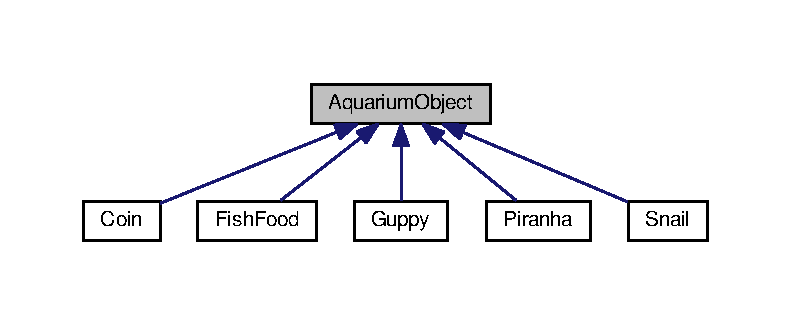
\includegraphics[width=350pt]{class_aquarium_object__inherit__graph}
\end{center}
\end{figure}
\subsection*{Public Member Functions}
\begin{DoxyCompactItemize}
\item 
void \mbox{\hyperlink{class_aquarium_object_a5ab79d2c1c8eb52e0857b734803a7385}{set\+Xi}} (final double pX)
\item 
void \mbox{\hyperlink{class_aquarium_object_a9bd7deefac91c170bcdc15c823184193}{set\+Yi}} (final double pY)
\item 
double \mbox{\hyperlink{class_aquarium_object_a020f612b6195b3332a4bb602f9f098be}{get\+Xi}} ()
\item 
double \mbox{\hyperlink{class_aquarium_object_acc1d2d6ed24f6802eaded313d25785a8}{get\+Yi}} ()
\end{DoxyCompactItemize}


\subsection{Detailed Description}
Class \mbox{\hyperlink{class_aquarium_object}{Aquarium\+Object}}. This class is used as the abstraction class for another aquarium objects for example\+: \mbox{\hyperlink{class_guppy}{Guppy}}, \mbox{\hyperlink{class_piranha}{Piranha}}, \mbox{\hyperlink{class_snail}{Snail}}, \mbox{\hyperlink{class_fish_food}{Fish\+Food}}, etc 

\subsection{Member Function Documentation}
\mbox{\Hypertarget{class_aquarium_object_a020f612b6195b3332a4bb602f9f098be}\label{class_aquarium_object_a020f612b6195b3332a4bb602f9f098be}} 
\index{Aquarium\+Object@{Aquarium\+Object}!get\+Xi@{get\+Xi}}
\index{get\+Xi@{get\+Xi}!Aquarium\+Object@{Aquarium\+Object}}
\subsubsection{\texorpdfstring{get\+Xi()}{getXi()}}
{\footnotesize\ttfamily double Aquarium\+Object.\+get\+Xi (\begin{DoxyParamCaption}{ }\end{DoxyParamCaption})\hspace{0.3cm}{\ttfamily [inline]}}

Get abscissa.

\begin{DoxyReturn}{Returns}
abscissa 
\end{DoxyReturn}
\mbox{\Hypertarget{class_aquarium_object_acc1d2d6ed24f6802eaded313d25785a8}\label{class_aquarium_object_acc1d2d6ed24f6802eaded313d25785a8}} 
\index{Aquarium\+Object@{Aquarium\+Object}!get\+Yi@{get\+Yi}}
\index{get\+Yi@{get\+Yi}!Aquarium\+Object@{Aquarium\+Object}}
\subsubsection{\texorpdfstring{get\+Yi()}{getYi()}}
{\footnotesize\ttfamily double Aquarium\+Object.\+get\+Yi (\begin{DoxyParamCaption}{ }\end{DoxyParamCaption})\hspace{0.3cm}{\ttfamily [inline]}}

Get ordinate.

\begin{DoxyReturn}{Returns}
ordinate 
\end{DoxyReturn}
\mbox{\Hypertarget{class_aquarium_object_a5ab79d2c1c8eb52e0857b734803a7385}\label{class_aquarium_object_a5ab79d2c1c8eb52e0857b734803a7385}} 
\index{Aquarium\+Object@{Aquarium\+Object}!set\+Xi@{set\+Xi}}
\index{set\+Xi@{set\+Xi}!Aquarium\+Object@{Aquarium\+Object}}
\subsubsection{\texorpdfstring{set\+Xi()}{setXi()}}
{\footnotesize\ttfamily void Aquarium\+Object.\+set\+Xi (\begin{DoxyParamCaption}\item[{final double}]{pX }\end{DoxyParamCaption})\hspace{0.3cm}{\ttfamily [inline]}}

Set the abscissa.


\begin{DoxyParams}{Parameters}
{\em pX} & is the abscissa \\
\hline
\end{DoxyParams}
\mbox{\Hypertarget{class_aquarium_object_a9bd7deefac91c170bcdc15c823184193}\label{class_aquarium_object_a9bd7deefac91c170bcdc15c823184193}} 
\index{Aquarium\+Object@{Aquarium\+Object}!set\+Yi@{set\+Yi}}
\index{set\+Yi@{set\+Yi}!Aquarium\+Object@{Aquarium\+Object}}
\subsubsection{\texorpdfstring{set\+Yi()}{setYi()}}
{\footnotesize\ttfamily void Aquarium\+Object.\+set\+Yi (\begin{DoxyParamCaption}\item[{final double}]{pY }\end{DoxyParamCaption})\hspace{0.3cm}{\ttfamily [inline]}}

Set the ordinate.


\begin{DoxyParams}{Parameters}
{\em pY} & is the ordinate \\
\hline
\end{DoxyParams}


The documentation for this class was generated from the following file\+:\begin{DoxyCompactItemize}
\item 
/media/malfianrasyidin/\+A\+L\+F\+I\+A\+N/java/\+Arkav\+Quarium\+Java/src/Aquarium\+Object.\+java\end{DoxyCompactItemize}

\hypertarget{class_coin}{}\section{Coin Class Reference}
\label{class_coin}\index{Coin@{Coin}}


Inheritance diagram for Coin\+:
\nopagebreak
\begin{figure}[H]
\begin{center}
\leavevmode
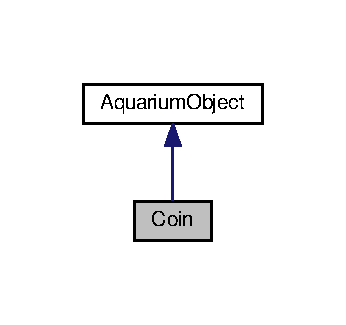
\includegraphics[width=166pt]{class_coin__inherit__graph}
\end{center}
\end{figure}


Collaboration diagram for Coin\+:
\nopagebreak
\begin{figure}[H]
\begin{center}
\leavevmode
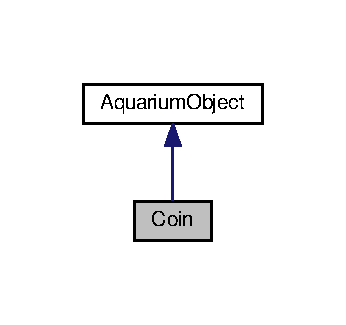
\includegraphics[width=166pt]{class_coin__coll__graph}
\end{center}
\end{figure}
\subsection*{Public Member Functions}
\begin{DoxyCompactItemize}
\item 
void \mbox{\hyperlink{class_coin_a649f0d0db3acec80ad9d3967f8d272f1}{move}} (final Graphics g)
\end{DoxyCompactItemize}
\subsection*{Static Public Member Functions}
\begin{DoxyCompactItemize}
\item 
static void \mbox{\hyperlink{class_coin_a64f7031c90885f5b2968f0ec9416b5a6}{set\+Image\+Coin}} (final Buffered\+Image p\+Image\+Coin)
\item 
static void \mbox{\hyperlink{class_coin_a10e0cd7c1b10e16149d3fb475ce8f1fd}{set\+Image\+Diamond}} (final Buffered\+Image p\+Image\+Diamond)
\item 
static void \mbox{\hyperlink{class_coin_afd75c4b3e2880aaed0bf3ced9ebc2704}{set\+List\+Coin}} (final \mbox{\hyperlink{class_linked_list}{Linked\+List}}$<$ \mbox{\hyperlink{class_coin}{Coin}} $>$ p\+List\+Coin)
\item 
static \mbox{\hyperlink{class_linked_list}{Linked\+List}}$<$ \mbox{\hyperlink{class_coin}{Coin}} $>$ \mbox{\hyperlink{class_coin_a9e49a7cd1e81f67f7664a0619242840f}{get\+List\+Coin}} ()
\end{DoxyCompactItemize}


\subsection{Detailed Description}
Class \mbox{\hyperlink{class_coin}{Coin}}. This class is derived from \mbox{\hyperlink{class_aquarium_object}{Aquarium\+Object}} and used for instantiate coins in the game in order to increase money. Furthermore, coins are produced by all derived class of \mbox{\hyperlink{interface_fish}{Fish}} 

\subsection{Member Function Documentation}
\mbox{\Hypertarget{class_coin_a9e49a7cd1e81f67f7664a0619242840f}\label{class_coin_a9e49a7cd1e81f67f7664a0619242840f}} 
\index{Coin@{Coin}!get\+List\+Coin@{get\+List\+Coin}}
\index{get\+List\+Coin@{get\+List\+Coin}!Coin@{Coin}}
\subsubsection{\texorpdfstring{get\+List\+Coin()}{getListCoin()}}
{\footnotesize\ttfamily static \mbox{\hyperlink{class_linked_list}{Linked\+List}}$<$\mbox{\hyperlink{class_coin}{Coin}}$>$ Coin.\+get\+List\+Coin (\begin{DoxyParamCaption}{ }\end{DoxyParamCaption})\hspace{0.3cm}{\ttfamily [inline]}, {\ttfamily [static]}}

Get list of coin.

\begin{DoxyReturn}{Returns}
the list of coin 
\end{DoxyReturn}
\mbox{\Hypertarget{class_coin_a649f0d0db3acec80ad9d3967f8d272f1}\label{class_coin_a649f0d0db3acec80ad9d3967f8d272f1}} 
\index{Coin@{Coin}!move@{move}}
\index{move@{move}!Coin@{Coin}}
\subsubsection{\texorpdfstring{move()}{move()}}
{\footnotesize\ttfamily void Coin.\+move (\begin{DoxyParamCaption}\item[{final Graphics}]{g }\end{DoxyParamCaption})\hspace{0.3cm}{\ttfamily [inline]}}

\mbox{\hyperlink{class_coin}{Coin}} is moving down as free fall. After it reaches ground, it will stop.


\begin{DoxyParams}{Parameters}
{\em g} & is the Graphics \\
\hline
\end{DoxyParams}
\mbox{\Hypertarget{class_coin_a64f7031c90885f5b2968f0ec9416b5a6}\label{class_coin_a64f7031c90885f5b2968f0ec9416b5a6}} 
\index{Coin@{Coin}!set\+Image\+Coin@{set\+Image\+Coin}}
\index{set\+Image\+Coin@{set\+Image\+Coin}!Coin@{Coin}}
\subsubsection{\texorpdfstring{set\+Image\+Coin()}{setImageCoin()}}
{\footnotesize\ttfamily static void Coin.\+set\+Image\+Coin (\begin{DoxyParamCaption}\item[{final Buffered\+Image}]{p\+Image\+Coin }\end{DoxyParamCaption})\hspace{0.3cm}{\ttfamily [inline]}, {\ttfamily [static]}}

Set image of coin.


\begin{DoxyParams}{Parameters}
{\em p\+Image\+Coin} & is the Buffered\+Image \\
\hline
\end{DoxyParams}
\mbox{\Hypertarget{class_coin_a10e0cd7c1b10e16149d3fb475ce8f1fd}\label{class_coin_a10e0cd7c1b10e16149d3fb475ce8f1fd}} 
\index{Coin@{Coin}!set\+Image\+Diamond@{set\+Image\+Diamond}}
\index{set\+Image\+Diamond@{set\+Image\+Diamond}!Coin@{Coin}}
\subsubsection{\texorpdfstring{set\+Image\+Diamond()}{setImageDiamond()}}
{\footnotesize\ttfamily static void Coin.\+set\+Image\+Diamond (\begin{DoxyParamCaption}\item[{final Buffered\+Image}]{p\+Image\+Diamond }\end{DoxyParamCaption})\hspace{0.3cm}{\ttfamily [inline]}, {\ttfamily [static]}}

Set image of diamond.


\begin{DoxyParams}{Parameters}
{\em p\+Image\+Diamond} & is the Buffered\+Image \\
\hline
\end{DoxyParams}
\mbox{\Hypertarget{class_coin_afd75c4b3e2880aaed0bf3ced9ebc2704}\label{class_coin_afd75c4b3e2880aaed0bf3ced9ebc2704}} 
\index{Coin@{Coin}!set\+List\+Coin@{set\+List\+Coin}}
\index{set\+List\+Coin@{set\+List\+Coin}!Coin@{Coin}}
\subsubsection{\texorpdfstring{set\+List\+Coin()}{setListCoin()}}
{\footnotesize\ttfamily static void Coin.\+set\+List\+Coin (\begin{DoxyParamCaption}\item[{final \mbox{\hyperlink{class_linked_list}{Linked\+List}}$<$ \mbox{\hyperlink{class_coin}{Coin}} $>$}]{p\+List\+Coin }\end{DoxyParamCaption})\hspace{0.3cm}{\ttfamily [inline]}, {\ttfamily [static]}}

Set list of coin.


\begin{DoxyParams}{Parameters}
{\em p\+List\+Coin} & is the list coin \\
\hline
\end{DoxyParams}


The documentation for this class was generated from the following file\+:\begin{DoxyCompactItemize}
\item 
/media/malfianrasyidin/\+A\+L\+F\+I\+A\+N/java/\+Arkav\+Quarium\+Java/src/Coin.\+java\end{DoxyCompactItemize}

\hypertarget{interface_fish}{}\section{Fish Interface Reference}
\label{interface_fish}\index{Fish@{Fish}}


Inheritance diagram for Fish\+:
\nopagebreak
\begin{figure}[H]
\begin{center}
\leavevmode
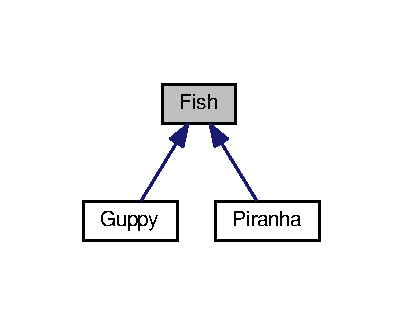
\includegraphics[width=194pt]{interface_fish__inherit__graph}
\end{center}
\end{figure}
\subsection*{Public Member Functions}
\begin{DoxyCompactItemize}
\item 
void \mbox{\hyperlink{interface_fish_a72d533bdc4ac39f4ffd93d70504efed8}{eat}} ()
\item 
void \mbox{\hyperlink{interface_fish_ad37facd4d5859411cf433520f03ae0b8}{drop\+Coin}} ()
\end{DoxyCompactItemize}


\subsection{Detailed Description}
Interface \mbox{\hyperlink{interface_fish}{Fish}}. This interface is used to defined the \mbox{\hyperlink{interface_fish}{Fish}} object. 

\subsection{Member Function Documentation}
\mbox{\Hypertarget{interface_fish_ad37facd4d5859411cf433520f03ae0b8}\label{interface_fish_ad37facd4d5859411cf433520f03ae0b8}} 
\index{Fish@{Fish}!drop\+Coin@{drop\+Coin}}
\index{drop\+Coin@{drop\+Coin}!Fish@{Fish}}
\subsubsection{\texorpdfstring{drop\+Coin()}{dropCoin()}}
{\footnotesize\ttfamily void Fish.\+drop\+Coin (\begin{DoxyParamCaption}{ }\end{DoxyParamCaption})}

This method used to drop the coin. 

Implemented in \mbox{\hyperlink{class_guppy_ace5750be512718d97f184f6ede72d25f}{Guppy}}, and \mbox{\hyperlink{class_piranha_ac7d4af6cc29513e5bd351cbbaf25cc0b}{Piranha}}.

\mbox{\Hypertarget{interface_fish_a72d533bdc4ac39f4ffd93d70504efed8}\label{interface_fish_a72d533bdc4ac39f4ffd93d70504efed8}} 
\index{Fish@{Fish}!eat@{eat}}
\index{eat@{eat}!Fish@{Fish}}
\subsubsection{\texorpdfstring{eat()}{eat()}}
{\footnotesize\ttfamily void Fish.\+eat (\begin{DoxyParamCaption}{ }\end{DoxyParamCaption})}

This method represents the action of eating. 

Implemented in \mbox{\hyperlink{class_guppy_a8cae34f3e9f4011e41da1d098363f1fc}{Guppy}}, and \mbox{\hyperlink{class_piranha_ac9bde9a286096cf199bdb1df5434a8c8}{Piranha}}.



The documentation for this interface was generated from the following file\+:\begin{DoxyCompactItemize}
\item 
/media/malfianrasyidin/\+A\+L\+F\+I\+A\+N/java/\+Arkav\+Quarium\+Java/src/Fish.\+java\end{DoxyCompactItemize}

\hypertarget{class_fish_food}{}\section{Fish\+Food Class Reference}
\label{class_fish_food}\index{Fish\+Food@{Fish\+Food}}


Inheritance diagram for Fish\+Food\+:
\nopagebreak
\begin{figure}[H]
\begin{center}
\leavevmode
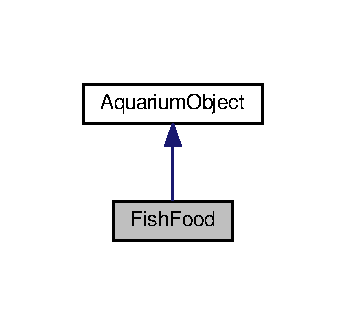
\includegraphics[width=166pt]{class_fish_food__inherit__graph}
\end{center}
\end{figure}


Collaboration diagram for Fish\+Food\+:
\nopagebreak
\begin{figure}[H]
\begin{center}
\leavevmode
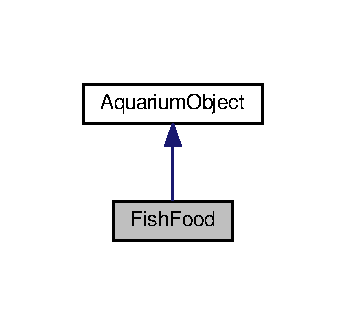
\includegraphics[width=166pt]{class_fish_food__coll__graph}
\end{center}
\end{figure}
\subsection*{Public Member Functions}
\begin{DoxyCompactItemize}
\item 
\mbox{\hyperlink{class_fish_food_aa3c6283b8dcbf8fc6343051bb2cbb522}{Fish\+Food}} (final double x, final double y)
\item 
double \mbox{\hyperlink{class_fish_food_a2b498cda505d338c12ef59f7d4746325}{get\+Radius}} ()
\item 
void \mbox{\hyperlink{class_fish_food_a0e72b850cf4211a1613e0376bf2d286e}{move}} (final Graphics g)
\end{DoxyCompactItemize}
\subsection*{Static Public Member Functions}
\begin{DoxyCompactItemize}
\item 
static void \mbox{\hyperlink{class_fish_food_a47a9051f2151bcbd87da5f07492bb6c9}{set\+Image}} (final Buffered\+Image p\+Image)
\item 
static void \mbox{\hyperlink{class_fish_food_ab2ad298b74bf3d3d0104ce0cffbaf7ff}{set\+List\+Fish\+Food}} (final \mbox{\hyperlink{class_linked_list}{Linked\+List}}$<$ \mbox{\hyperlink{class_fish_food}{Fish\+Food}} $>$ p\+List\+Fish\+Food)
\item 
static double \mbox{\hyperlink{class_fish_food_a70b3341a3d7018ed280e8e079806f3a0}{get\+Velocity}} ()
\item 
static \mbox{\hyperlink{class_linked_list}{Linked\+List}}$<$ \mbox{\hyperlink{class_fish_food}{Fish\+Food}} $>$ \mbox{\hyperlink{class_fish_food_aa35d784e5f8c59d1029fcb119eaf302b}{get\+List\+Fish\+Food}} ()
\end{DoxyCompactItemize}


\subsection{Detailed Description}
Class \mbox{\hyperlink{class_fish_food}{Fish\+Food}}. This class is derived from \mbox{\hyperlink{class_aquarium_object}{Aquarium\+Object}}. It is used as the food of \mbox{\hyperlink{class_guppy}{Guppy}} -\/ a derived \mbox{\hyperlink{interface_fish}{Fish}} object. \mbox{\hyperlink{class_fish_food}{Fish\+Food}} is bought by the player using the coin while the game is running. 

\subsection{Constructor \& Destructor Documentation}
\mbox{\Hypertarget{class_fish_food_aa3c6283b8dcbf8fc6343051bb2cbb522}\label{class_fish_food_aa3c6283b8dcbf8fc6343051bb2cbb522}} 
\index{Fish\+Food@{Fish\+Food}!Fish\+Food@{Fish\+Food}}
\index{Fish\+Food@{Fish\+Food}!Fish\+Food@{Fish\+Food}}
\subsubsection{\texorpdfstring{Fish\+Food()}{FishFood()}}
{\footnotesize\ttfamily Fish\+Food.\+Fish\+Food (\begin{DoxyParamCaption}\item[{final double}]{x,  }\item[{final double}]{y }\end{DoxyParamCaption})\hspace{0.3cm}{\ttfamily [inline]}}

Instantiate \mbox{\hyperlink{class_fish_food}{Fish\+Food}}.


\begin{DoxyParams}{Parameters}
{\em x} & is the abscissa \\
\hline
{\em y} & is the ordinate \\
\hline
\end{DoxyParams}


\subsection{Member Function Documentation}
\mbox{\Hypertarget{class_fish_food_aa35d784e5f8c59d1029fcb119eaf302b}\label{class_fish_food_aa35d784e5f8c59d1029fcb119eaf302b}} 
\index{Fish\+Food@{Fish\+Food}!get\+List\+Fish\+Food@{get\+List\+Fish\+Food}}
\index{get\+List\+Fish\+Food@{get\+List\+Fish\+Food}!Fish\+Food@{Fish\+Food}}
\subsubsection{\texorpdfstring{get\+List\+Fish\+Food()}{getListFishFood()}}
{\footnotesize\ttfamily static \mbox{\hyperlink{class_linked_list}{Linked\+List}}$<$\mbox{\hyperlink{class_fish_food}{Fish\+Food}}$>$ Fish\+Food.\+get\+List\+Fish\+Food (\begin{DoxyParamCaption}{ }\end{DoxyParamCaption})\hspace{0.3cm}{\ttfamily [inline]}, {\ttfamily [static]}}

Get list of \mbox{\hyperlink{class_fish_food}{Fish\+Food}}.

\begin{DoxyReturn}{Returns}
list\+Fish\+Food list fish food 
\end{DoxyReturn}
\mbox{\Hypertarget{class_fish_food_a2b498cda505d338c12ef59f7d4746325}\label{class_fish_food_a2b498cda505d338c12ef59f7d4746325}} 
\index{Fish\+Food@{Fish\+Food}!get\+Radius@{get\+Radius}}
\index{get\+Radius@{get\+Radius}!Fish\+Food@{Fish\+Food}}
\subsubsection{\texorpdfstring{get\+Radius()}{getRadius()}}
{\footnotesize\ttfamily double Fish\+Food.\+get\+Radius (\begin{DoxyParamCaption}{ }\end{DoxyParamCaption})\hspace{0.3cm}{\ttfamily [inline]}}

Get radius.

\begin{DoxyReturn}{Returns}
radius 
\end{DoxyReturn}
\mbox{\Hypertarget{class_fish_food_a70b3341a3d7018ed280e8e079806f3a0}\label{class_fish_food_a70b3341a3d7018ed280e8e079806f3a0}} 
\index{Fish\+Food@{Fish\+Food}!get\+Velocity@{get\+Velocity}}
\index{get\+Velocity@{get\+Velocity}!Fish\+Food@{Fish\+Food}}
\subsubsection{\texorpdfstring{get\+Velocity()}{getVelocity()}}
{\footnotesize\ttfamily static double Fish\+Food.\+get\+Velocity (\begin{DoxyParamCaption}{ }\end{DoxyParamCaption})\hspace{0.3cm}{\ttfamily [inline]}, {\ttfamily [static]}}

Get velocity.

\begin{DoxyReturn}{Returns}
velocity 
\end{DoxyReturn}
\mbox{\Hypertarget{class_fish_food_a0e72b850cf4211a1613e0376bf2d286e}\label{class_fish_food_a0e72b850cf4211a1613e0376bf2d286e}} 
\index{Fish\+Food@{Fish\+Food}!move@{move}}
\index{move@{move}!Fish\+Food@{Fish\+Food}}
\subsubsection{\texorpdfstring{move()}{move()}}
{\footnotesize\ttfamily void Fish\+Food.\+move (\begin{DoxyParamCaption}\item[{final Graphics}]{g }\end{DoxyParamCaption})\hspace{0.3cm}{\ttfamily [inline]}}

\mbox{\hyperlink{class_fish_food}{Fish\+Food}} is moving down as free fall. After it reaches ground, it will disappear.


\begin{DoxyParams}{Parameters}
{\em g} & is the Graphics \\
\hline
\end{DoxyParams}
\mbox{\Hypertarget{class_fish_food_a47a9051f2151bcbd87da5f07492bb6c9}\label{class_fish_food_a47a9051f2151bcbd87da5f07492bb6c9}} 
\index{Fish\+Food@{Fish\+Food}!set\+Image@{set\+Image}}
\index{set\+Image@{set\+Image}!Fish\+Food@{Fish\+Food}}
\subsubsection{\texorpdfstring{set\+Image()}{setImage()}}
{\footnotesize\ttfamily static void Fish\+Food.\+set\+Image (\begin{DoxyParamCaption}\item[{final Buffered\+Image}]{p\+Image }\end{DoxyParamCaption})\hspace{0.3cm}{\ttfamily [inline]}, {\ttfamily [static]}}

Set image of \mbox{\hyperlink{class_fish_food}{Fish\+Food}}.


\begin{DoxyParams}{Parameters}
{\em p\+Image} & is Buffered\+Image \\
\hline
\end{DoxyParams}
\mbox{\Hypertarget{class_fish_food_ab2ad298b74bf3d3d0104ce0cffbaf7ff}\label{class_fish_food_ab2ad298b74bf3d3d0104ce0cffbaf7ff}} 
\index{Fish\+Food@{Fish\+Food}!set\+List\+Fish\+Food@{set\+List\+Fish\+Food}}
\index{set\+List\+Fish\+Food@{set\+List\+Fish\+Food}!Fish\+Food@{Fish\+Food}}
\subsubsection{\texorpdfstring{set\+List\+Fish\+Food()}{setListFishFood()}}
{\footnotesize\ttfamily static void Fish\+Food.\+set\+List\+Fish\+Food (\begin{DoxyParamCaption}\item[{final \mbox{\hyperlink{class_linked_list}{Linked\+List}}$<$ \mbox{\hyperlink{class_fish_food}{Fish\+Food}} $>$}]{p\+List\+Fish\+Food }\end{DoxyParamCaption})\hspace{0.3cm}{\ttfamily [inline]}, {\ttfamily [static]}}

Set list of fish food.


\begin{DoxyParams}{Parameters}
{\em p\+List\+Fish\+Food} & is the list of \mbox{\hyperlink{class_fish_food}{Fish\+Food}} \\
\hline
\end{DoxyParams}


The documentation for this class was generated from the following file\+:\begin{DoxyCompactItemize}
\item 
/media/malfianrasyidin/\+A\+L\+F\+I\+A\+N/java/\+Arkav\+Quarium\+Java/src/Fish\+Food.\+java\end{DoxyCompactItemize}

\hypertarget{class_guppy}{}\section{Guppy Class Reference}
\label{class_guppy}\index{Guppy@{Guppy}}


Inheritance diagram for Guppy\+:
\nopagebreak
\begin{figure}[H]
\begin{center}
\leavevmode
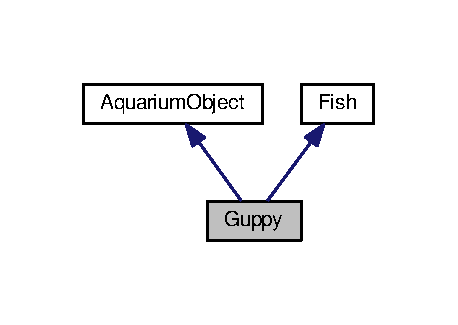
\includegraphics[width=220pt]{class_guppy__inherit__graph}
\end{center}
\end{figure}


Collaboration diagram for Guppy\+:
\nopagebreak
\begin{figure}[H]
\begin{center}
\leavevmode
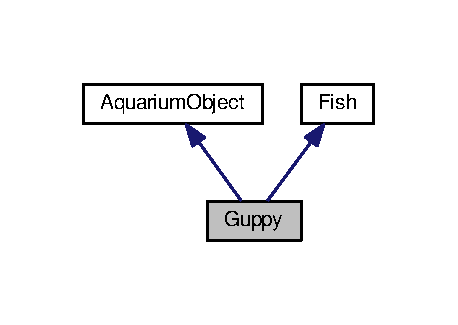
\includegraphics[width=220pt]{class_guppy__coll__graph}
\end{center}
\end{figure}
\subsection*{Public Member Functions}
\begin{DoxyCompactItemize}
\item 
\mbox{\hyperlink{class_guppy_a6336822c9cc2106fad2aaa2e54d159ac}{Guppy}} ()
\item 
void \mbox{\hyperlink{class_guppy_a8cae34f3e9f4011e41da1d098363f1fc}{eat}} ()
\item 
void \mbox{\hyperlink{class_guppy_ace5750be512718d97f184f6ede72d25f}{drop\+Coin}} ()
\end{DoxyCompactItemize}
\subsection*{Static Public Member Functions}
\begin{DoxyCompactItemize}
\item 
static void \mbox{\hyperlink{class_guppy_a46004a42a6bea1e8fce0f26a61351d17}{set\+List\+Coin}} (final \mbox{\hyperlink{class_linked_list}{Linked\+List}}$<$ \mbox{\hyperlink{class_coin}{Coin}} $>$ p\+List\+Coin)
\item 
static void \mbox{\hyperlink{class_guppy_a87b2657fb98da613855fc016efa5e9d5}{set\+List\+Guppy}} (final \mbox{\hyperlink{class_linked_list}{Linked\+List}}$<$ \mbox{\hyperlink{class_guppy}{Guppy}} $>$ p\+List\+Guppy)
\item 
static void \mbox{\hyperlink{class_guppy_acc235342cdaa86c847ab01eb55043d7e}{set\+List\+Fish\+Food}} (final \mbox{\hyperlink{class_linked_list}{Linked\+List}}$<$ \mbox{\hyperlink{class_fish_food}{Fish\+Food}} $>$ p\+List\+Fish\+Food)
\item 
static void \mbox{\hyperlink{class_guppy_a9a8f6225f0482e0bd57a81f51310257c}{set\+State\+One\+Guppy\+Left}} (final Buffered\+Image p\+State\+One\+Guppy\+Left)
\item 
static void \mbox{\hyperlink{class_guppy_a49fdfd0f9d8e9eacbb032a0e16b67db0}{set\+State\+One\+Guppy\+Right}} (final Buffered\+Image p\+State\+One\+Guppy\+Right)
\item 
static void \mbox{\hyperlink{class_guppy_a7f916a9190171f6311d2404913fb2df6}{set\+State\+Two\+Guppy\+Left}} (final Buffered\+Image p\+State\+Two\+Guppy\+Left)
\item 
static void \mbox{\hyperlink{class_guppy_a17a6b8605b82965f1e6c290aa12da7a6}{set\+State\+Two\+Guppy\+Right}} (final Buffered\+Image p\+State\+Two\+Guppy\+Right)
\item 
static void \mbox{\hyperlink{class_guppy_ad66c660e52a40d1f10398c04b3a72d2c}{set\+State\+Three\+Guppy\+Left}} (final Buffered\+Image p\+State\+Three\+Guppy\+Left)
\item 
static void \mbox{\hyperlink{class_guppy_aff40345fa3a3ace95695a3bad8ebe1a5}{set\+State\+Three\+Guppy\+Right}} (final Buffered\+Image p\+State\+Three\+Guppy\+Right)
\end{DoxyCompactItemize}


\subsection{Detailed Description}
Class \mbox{\hyperlink{class_guppy}{Guppy}}. This class is derived from \mbox{\hyperlink{class_aquarium_object}{Aquarium\+Object}}. \mbox{\hyperlink{class_guppy}{Guppy}} is an aquarium object than can be bought during the game using the coins that the player has. It also can drop coins in a regular interval of time with variety of value. 

\subsection{Constructor \& Destructor Documentation}
\mbox{\Hypertarget{class_guppy_a6336822c9cc2106fad2aaa2e54d159ac}\label{class_guppy_a6336822c9cc2106fad2aaa2e54d159ac}} 
\index{Guppy@{Guppy}!Guppy@{Guppy}}
\index{Guppy@{Guppy}!Guppy@{Guppy}}
\subsubsection{\texorpdfstring{Guppy()}{Guppy()}}
{\footnotesize\ttfamily Guppy.\+Guppy (\begin{DoxyParamCaption}{ }\end{DoxyParamCaption})\hspace{0.3cm}{\ttfamily [inline]}}

Instantiate \mbox{\hyperlink{class_guppy}{Guppy}}. 

\subsection{Member Function Documentation}
\mbox{\Hypertarget{class_guppy_ace5750be512718d97f184f6ede72d25f}\label{class_guppy_ace5750be512718d97f184f6ede72d25f}} 
\index{Guppy@{Guppy}!drop\+Coin@{drop\+Coin}}
\index{drop\+Coin@{drop\+Coin}!Guppy@{Guppy}}
\subsubsection{\texorpdfstring{drop\+Coin()}{dropCoin()}}
{\footnotesize\ttfamily void Guppy.\+drop\+Coin (\begin{DoxyParamCaption}{ }\end{DoxyParamCaption})\hspace{0.3cm}{\ttfamily [inline]}}

This method will drop coin. \mbox{\hyperlink{class_coin}{Coin}} will drop regularly based on certain interval. Also, coin value calculated from the multiplication of C\+O\+I\+N\+\_\+\+D\+R\+O\+P\+\_\+\+V\+A\+L\+UE and state 

Implements \mbox{\hyperlink{interface_fish_ad37facd4d5859411cf433520f03ae0b8}{Fish}}.

\mbox{\Hypertarget{class_guppy_a8cae34f3e9f4011e41da1d098363f1fc}\label{class_guppy_a8cae34f3e9f4011e41da1d098363f1fc}} 
\index{Guppy@{Guppy}!eat@{eat}}
\index{eat@{eat}!Guppy@{Guppy}}
\subsubsection{\texorpdfstring{eat()}{eat()}}
{\footnotesize\ttfamily void Guppy.\+eat (\begin{DoxyParamCaption}{ }\end{DoxyParamCaption})\hspace{0.3cm}{\ttfamily [inline]}}

This method will eat \mbox{\hyperlink{class_fish_food}{Fish\+Food}}. \mbox{\hyperlink{class_guppy}{Guppy}} only eats when \mbox{\hyperlink{class_guppy}{Guppy}} is hungry and will try to reach the nearest food available. 

Implements \mbox{\hyperlink{interface_fish_a72d533bdc4ac39f4ffd93d70504efed8}{Fish}}.

\mbox{\Hypertarget{class_guppy_a46004a42a6bea1e8fce0f26a61351d17}\label{class_guppy_a46004a42a6bea1e8fce0f26a61351d17}} 
\index{Guppy@{Guppy}!set\+List\+Coin@{set\+List\+Coin}}
\index{set\+List\+Coin@{set\+List\+Coin}!Guppy@{Guppy}}
\subsubsection{\texorpdfstring{set\+List\+Coin()}{setListCoin()}}
{\footnotesize\ttfamily static void Guppy.\+set\+List\+Coin (\begin{DoxyParamCaption}\item[{final \mbox{\hyperlink{class_linked_list}{Linked\+List}}$<$ \mbox{\hyperlink{class_coin}{Coin}} $>$}]{p\+List\+Coin }\end{DoxyParamCaption})\hspace{0.3cm}{\ttfamily [inline]}, {\ttfamily [static]}}

Set list of coins.


\begin{DoxyParams}{Parameters}
{\em p\+List\+Coin} & is list of coins \\
\hline
\end{DoxyParams}
\mbox{\Hypertarget{class_guppy_acc235342cdaa86c847ab01eb55043d7e}\label{class_guppy_acc235342cdaa86c847ab01eb55043d7e}} 
\index{Guppy@{Guppy}!set\+List\+Fish\+Food@{set\+List\+Fish\+Food}}
\index{set\+List\+Fish\+Food@{set\+List\+Fish\+Food}!Guppy@{Guppy}}
\subsubsection{\texorpdfstring{set\+List\+Fish\+Food()}{setListFishFood()}}
{\footnotesize\ttfamily static void Guppy.\+set\+List\+Fish\+Food (\begin{DoxyParamCaption}\item[{final \mbox{\hyperlink{class_linked_list}{Linked\+List}}$<$ \mbox{\hyperlink{class_fish_food}{Fish\+Food}} $>$}]{p\+List\+Fish\+Food }\end{DoxyParamCaption})\hspace{0.3cm}{\ttfamily [inline]}, {\ttfamily [static]}}

Set list of \mbox{\hyperlink{class_fish_food}{Fish\+Food}}.


\begin{DoxyParams}{Parameters}
{\em p\+List\+Fish\+Food} & is list of \mbox{\hyperlink{class_fish_food}{Fish\+Food}} \\
\hline
\end{DoxyParams}
\mbox{\Hypertarget{class_guppy_a87b2657fb98da613855fc016efa5e9d5}\label{class_guppy_a87b2657fb98da613855fc016efa5e9d5}} 
\index{Guppy@{Guppy}!set\+List\+Guppy@{set\+List\+Guppy}}
\index{set\+List\+Guppy@{set\+List\+Guppy}!Guppy@{Guppy}}
\subsubsection{\texorpdfstring{set\+List\+Guppy()}{setListGuppy()}}
{\footnotesize\ttfamily static void Guppy.\+set\+List\+Guppy (\begin{DoxyParamCaption}\item[{final \mbox{\hyperlink{class_linked_list}{Linked\+List}}$<$ \mbox{\hyperlink{class_guppy}{Guppy}} $>$}]{p\+List\+Guppy }\end{DoxyParamCaption})\hspace{0.3cm}{\ttfamily [inline]}, {\ttfamily [static]}}

Set list of \mbox{\hyperlink{class_guppy}{Guppy}}.


\begin{DoxyParams}{Parameters}
{\em p\+List\+Guppy} & is list of \mbox{\hyperlink{class_guppy}{Guppy}} \\
\hline
\end{DoxyParams}
\mbox{\Hypertarget{class_guppy_a9a8f6225f0482e0bd57a81f51310257c}\label{class_guppy_a9a8f6225f0482e0bd57a81f51310257c}} 
\index{Guppy@{Guppy}!set\+State\+One\+Guppy\+Left@{set\+State\+One\+Guppy\+Left}}
\index{set\+State\+One\+Guppy\+Left@{set\+State\+One\+Guppy\+Left}!Guppy@{Guppy}}
\subsubsection{\texorpdfstring{set\+State\+One\+Guppy\+Left()}{setStateOneGuppyLeft()}}
{\footnotesize\ttfamily static void Guppy.\+set\+State\+One\+Guppy\+Left (\begin{DoxyParamCaption}\item[{final Buffered\+Image}]{p\+State\+One\+Guppy\+Left }\end{DoxyParamCaption})\hspace{0.3cm}{\ttfamily [inline]}, {\ttfamily [static]}}

Set image of \mbox{\hyperlink{class_guppy}{Guppy}}. \mbox{\hyperlink{class_guppy}{Guppy}} is on first level and facing left.


\begin{DoxyParams}{Parameters}
{\em p\+State\+One\+Guppy\+Left} & is Buffered\+Image \\
\hline
\end{DoxyParams}
\mbox{\Hypertarget{class_guppy_a49fdfd0f9d8e9eacbb032a0e16b67db0}\label{class_guppy_a49fdfd0f9d8e9eacbb032a0e16b67db0}} 
\index{Guppy@{Guppy}!set\+State\+One\+Guppy\+Right@{set\+State\+One\+Guppy\+Right}}
\index{set\+State\+One\+Guppy\+Right@{set\+State\+One\+Guppy\+Right}!Guppy@{Guppy}}
\subsubsection{\texorpdfstring{set\+State\+One\+Guppy\+Right()}{setStateOneGuppyRight()}}
{\footnotesize\ttfamily static void Guppy.\+set\+State\+One\+Guppy\+Right (\begin{DoxyParamCaption}\item[{final Buffered\+Image}]{p\+State\+One\+Guppy\+Right }\end{DoxyParamCaption})\hspace{0.3cm}{\ttfamily [inline]}, {\ttfamily [static]}}

Set image of \mbox{\hyperlink{class_guppy}{Guppy}}. \mbox{\hyperlink{class_guppy}{Guppy}} is on first level and facing right.


\begin{DoxyParams}{Parameters}
{\em p\+State\+One\+Guppy\+Right} & is Buffered\+Image \\
\hline
\end{DoxyParams}
\mbox{\Hypertarget{class_guppy_ad66c660e52a40d1f10398c04b3a72d2c}\label{class_guppy_ad66c660e52a40d1f10398c04b3a72d2c}} 
\index{Guppy@{Guppy}!set\+State\+Three\+Guppy\+Left@{set\+State\+Three\+Guppy\+Left}}
\index{set\+State\+Three\+Guppy\+Left@{set\+State\+Three\+Guppy\+Left}!Guppy@{Guppy}}
\subsubsection{\texorpdfstring{set\+State\+Three\+Guppy\+Left()}{setStateThreeGuppyLeft()}}
{\footnotesize\ttfamily static void Guppy.\+set\+State\+Three\+Guppy\+Left (\begin{DoxyParamCaption}\item[{final Buffered\+Image}]{p\+State\+Three\+Guppy\+Left }\end{DoxyParamCaption})\hspace{0.3cm}{\ttfamily [inline]}, {\ttfamily [static]}}

Set image of \mbox{\hyperlink{class_guppy}{Guppy}}. \mbox{\hyperlink{class_guppy}{Guppy}} is on third level and facing left.


\begin{DoxyParams}{Parameters}
{\em p\+State\+Three\+Guppy\+Left} & is Buffered\+Image \\
\hline
\end{DoxyParams}
\mbox{\Hypertarget{class_guppy_aff40345fa3a3ace95695a3bad8ebe1a5}\label{class_guppy_aff40345fa3a3ace95695a3bad8ebe1a5}} 
\index{Guppy@{Guppy}!set\+State\+Three\+Guppy\+Right@{set\+State\+Three\+Guppy\+Right}}
\index{set\+State\+Three\+Guppy\+Right@{set\+State\+Three\+Guppy\+Right}!Guppy@{Guppy}}
\subsubsection{\texorpdfstring{set\+State\+Three\+Guppy\+Right()}{setStateThreeGuppyRight()}}
{\footnotesize\ttfamily static void Guppy.\+set\+State\+Three\+Guppy\+Right (\begin{DoxyParamCaption}\item[{final Buffered\+Image}]{p\+State\+Three\+Guppy\+Right }\end{DoxyParamCaption})\hspace{0.3cm}{\ttfamily [inline]}, {\ttfamily [static]}}

Set image of \mbox{\hyperlink{class_guppy}{Guppy}}. \mbox{\hyperlink{class_guppy}{Guppy}} is on third level and facing right.


\begin{DoxyParams}{Parameters}
{\em p\+State\+Three\+Guppy\+Right} & is Buffered\+Image \\
\hline
\end{DoxyParams}
\mbox{\Hypertarget{class_guppy_a7f916a9190171f6311d2404913fb2df6}\label{class_guppy_a7f916a9190171f6311d2404913fb2df6}} 
\index{Guppy@{Guppy}!set\+State\+Two\+Guppy\+Left@{set\+State\+Two\+Guppy\+Left}}
\index{set\+State\+Two\+Guppy\+Left@{set\+State\+Two\+Guppy\+Left}!Guppy@{Guppy}}
\subsubsection{\texorpdfstring{set\+State\+Two\+Guppy\+Left()}{setStateTwoGuppyLeft()}}
{\footnotesize\ttfamily static void Guppy.\+set\+State\+Two\+Guppy\+Left (\begin{DoxyParamCaption}\item[{final Buffered\+Image}]{p\+State\+Two\+Guppy\+Left }\end{DoxyParamCaption})\hspace{0.3cm}{\ttfamily [inline]}, {\ttfamily [static]}}

Set image of \mbox{\hyperlink{class_guppy}{Guppy}}. \mbox{\hyperlink{class_guppy}{Guppy}} is on second level and facing left.


\begin{DoxyParams}{Parameters}
{\em p\+State\+Two\+Guppy\+Left} & is Buffered\+Image \\
\hline
\end{DoxyParams}
\mbox{\Hypertarget{class_guppy_a17a6b8605b82965f1e6c290aa12da7a6}\label{class_guppy_a17a6b8605b82965f1e6c290aa12da7a6}} 
\index{Guppy@{Guppy}!set\+State\+Two\+Guppy\+Right@{set\+State\+Two\+Guppy\+Right}}
\index{set\+State\+Two\+Guppy\+Right@{set\+State\+Two\+Guppy\+Right}!Guppy@{Guppy}}
\subsubsection{\texorpdfstring{set\+State\+Two\+Guppy\+Right()}{setStateTwoGuppyRight()}}
{\footnotesize\ttfamily static void Guppy.\+set\+State\+Two\+Guppy\+Right (\begin{DoxyParamCaption}\item[{final Buffered\+Image}]{p\+State\+Two\+Guppy\+Right }\end{DoxyParamCaption})\hspace{0.3cm}{\ttfamily [inline]}, {\ttfamily [static]}}

Set image of \mbox{\hyperlink{class_guppy}{Guppy}}. \mbox{\hyperlink{class_guppy}{Guppy}} is on second level and facing right.


\begin{DoxyParams}{Parameters}
{\em p\+State\+Two\+Guppy\+Right} & is Buffered\+Image \\
\hline
\end{DoxyParams}


The documentation for this class was generated from the following file\+:\begin{DoxyCompactItemize}
\item 
/media/malfianrasyidin/\+A\+L\+F\+I\+A\+N/java/\+Arkav\+Quarium\+Java/src/Guppy.\+java\end{DoxyCompactItemize}

\hypertarget{class_linked_list}{}\section{Linked\+List$<$ T $>$ Class Template Reference}
\label{class_linked_list}\index{Linked\+List$<$ T $>$@{Linked\+List$<$ T $>$}}
\subsection*{Public Member Functions}
\begin{DoxyCompactItemize}
\item 
T \mbox{\hyperlink{class_linked_list_a00c77b8619b458b47bfbbc53f3d14ce7}{get}} (final int idx)
\item 
int \mbox{\hyperlink{class_linked_list_acd5221f9ec3d5eafa37321d5ef0b9396}{get\+Count}} ()
\item 
boolean \mbox{\hyperlink{class_linked_list_aecae3d82587c52087a4f65d6c56900e2}{is\+Empty}} ()
\item 
void \mbox{\hyperlink{class_linked_list_ad4873babcc03951eafb5cc17daebbfaf}{remove}} (final T node)
\end{DoxyCompactItemize}


\subsection{Detailed Description}
Template class \mbox{\hyperlink{class_linked_list}{Linked\+List}}. This is a template class for \mbox{\hyperlink{class_linked_list}{Linked\+List}}.


\begin{DoxyParams}{Parameters}
{\em $<$\+T$>$} & is the parameter type \\
\hline
\end{DoxyParams}


\subsection{Member Function Documentation}
\mbox{\Hypertarget{class_linked_list_a00c77b8619b458b47bfbbc53f3d14ce7}\label{class_linked_list_a00c77b8619b458b47bfbbc53f3d14ce7}} 
\index{Linked\+List@{Linked\+List}!get@{get}}
\index{get@{get}!Linked\+List@{Linked\+List}}
\subsubsection{\texorpdfstring{get()}{get()}}
{\footnotesize\ttfamily T \mbox{\hyperlink{class_linked_list}{Linked\+List}}$<$ T $>$.get (\begin{DoxyParamCaption}\item[{final int}]{idx }\end{DoxyParamCaption})\hspace{0.3cm}{\ttfamily [inline]}}

Get the object.


\begin{DoxyParams}{Parameters}
{\em idx} & is the index \\
\hline
\end{DoxyParams}
\begin{DoxyReturn}{Returns}
is the T 
\end{DoxyReturn}
\mbox{\Hypertarget{class_linked_list_acd5221f9ec3d5eafa37321d5ef0b9396}\label{class_linked_list_acd5221f9ec3d5eafa37321d5ef0b9396}} 
\index{Linked\+List@{Linked\+List}!get\+Count@{get\+Count}}
\index{get\+Count@{get\+Count}!Linked\+List@{Linked\+List}}
\subsubsection{\texorpdfstring{get\+Count()}{getCount()}}
{\footnotesize\ttfamily int \mbox{\hyperlink{class_linked_list}{Linked\+List}}$<$ T $>$.get\+Count (\begin{DoxyParamCaption}{ }\end{DoxyParamCaption})\hspace{0.3cm}{\ttfamily [inline]}}

Get the total object in the \mbox{\hyperlink{class_linked_list}{Linked\+List}}.

\begin{DoxyReturn}{Returns}
integer that represents the total number of object in the \mbox{\hyperlink{class_linked_list}{Linked\+List}} 
\end{DoxyReturn}
\mbox{\Hypertarget{class_linked_list_aecae3d82587c52087a4f65d6c56900e2}\label{class_linked_list_aecae3d82587c52087a4f65d6c56900e2}} 
\index{Linked\+List@{Linked\+List}!is\+Empty@{is\+Empty}}
\index{is\+Empty@{is\+Empty}!Linked\+List@{Linked\+List}}
\subsubsection{\texorpdfstring{is\+Empty()}{isEmpty()}}
{\footnotesize\ttfamily boolean \mbox{\hyperlink{class_linked_list}{Linked\+List}}$<$ T $>$.is\+Empty (\begin{DoxyParamCaption}{ }\end{DoxyParamCaption})\hspace{0.3cm}{\ttfamily [inline]}}

This method is used to check whether the \mbox{\hyperlink{class_linked_list}{Linked\+List}} is empty or not.

\begin{DoxyReturn}{Returns}
T\+R\+UE if the list is empty, otherwise F\+A\+L\+SE 
\end{DoxyReturn}
\mbox{\Hypertarget{class_linked_list_ad4873babcc03951eafb5cc17daebbfaf}\label{class_linked_list_ad4873babcc03951eafb5cc17daebbfaf}} 
\index{Linked\+List@{Linked\+List}!remove@{remove}}
\index{remove@{remove}!Linked\+List@{Linked\+List}}
\subsubsection{\texorpdfstring{remove()}{remove()}}
{\footnotesize\ttfamily void \mbox{\hyperlink{class_linked_list}{Linked\+List}}$<$ T $>$.remove (\begin{DoxyParamCaption}\item[{final T}]{node }\end{DoxyParamCaption})\hspace{0.3cm}{\ttfamily [inline]}}

This method will remove the object that is passed in its \mbox{\hyperlink{class_linked_list}{Linked\+List}}.


\begin{DoxyParams}{Parameters}
{\em node} & is the T. \\
\hline
\end{DoxyParams}


The documentation for this class was generated from the following file\+:\begin{DoxyCompactItemize}
\item 
/media/malfianrasyidin/\+A\+L\+F\+I\+A\+N/java/\+Arkav\+Quarium\+Java/src/Linked\+List.\+java\end{DoxyCompactItemize}

\hypertarget{class_main}{}\section{Main Class Reference}
\label{class_main}\index{Main@{Main}}
\subsection*{Static Public Member Functions}
\begin{DoxyCompactItemize}
\item 
static void \mbox{\hyperlink{class_main_a1f077a378d17565d62958633da1a12b7}{main}} (final String\mbox{[}$\,$\mbox{]} args)
\end{DoxyCompactItemize}


\subsection{Detailed Description}
Class \mbox{\hyperlink{class_main}{Main}}. This is the controller class to run another classes during the game 

\subsection{Member Function Documentation}
\mbox{\Hypertarget{class_main_a1f077a378d17565d62958633da1a12b7}\label{class_main_a1f077a378d17565d62958633da1a12b7}} 
\index{Main@{Main}!main@{main}}
\index{main@{main}!Main@{Main}}
\subsubsection{\texorpdfstring{main()}{main()}}
{\footnotesize\ttfamily static void Main.\+main (\begin{DoxyParamCaption}\item[{final String \mbox{[}$\,$\mbox{]}}]{args }\end{DoxyParamCaption})\hspace{0.3cm}{\ttfamily [inline]}, {\ttfamily [static]}}

\mbox{\hyperlink{class_main}{Main}} program.


\begin{DoxyParams}{Parameters}
{\em args} & is array string when execute program from command line \\
\hline
\end{DoxyParams}


The documentation for this class was generated from the following file\+:\begin{DoxyCompactItemize}
\item 
/media/malfianrasyidin/\+A\+L\+F\+I\+A\+N/java/\+Arkav\+Quarium\+Java/src/Main.\+java\end{DoxyCompactItemize}

\hypertarget{class_node}{}\section{Node$<$ T $>$ Class Template Reference}
\label{class_node}\index{Node$<$ T $>$@{Node$<$ T $>$}}
\subsection*{Public Member Functions}
\begin{DoxyCompactItemize}
\item 
\mbox{\hyperlink{class_node_a692c4af3a3274febfa32e5cb9b8b109d}{Node}} (final T p\+Data)
\item 
void \mbox{\hyperlink{class_node_a3fe482188599b86b0a11239a47a88443}{set\+Next}} (final \mbox{\hyperlink{class_node}{Node}}$<$ T $>$ p\+Next)
\item 
void \mbox{\hyperlink{class_node_ad5da4ea9b4329014fa04989d77aa8fab}{set\+Data}} (final T p\+Data)
\item 
T \mbox{\hyperlink{class_node_ab2b3d985988d010de2e125417c04d063}{get\+Data}} ()
\item 
\mbox{\hyperlink{class_node}{Node}}$<$ T $>$ \mbox{\hyperlink{class_node_a2ec63a299666383d35bdde247fb7fb67}{get\+Next}} ()
\end{DoxyCompactItemize}


\subsection{Detailed Description}
Class \mbox{\hyperlink{class_node}{Node}}. This is a template class for \mbox{\hyperlink{class_node}{Node}}.


\begin{DoxyParams}{Parameters}
{\em $<$\+T$>$} & is the parameter type \\
\hline
\end{DoxyParams}


\subsection{Constructor \& Destructor Documentation}
\mbox{\Hypertarget{class_node_a692c4af3a3274febfa32e5cb9b8b109d}\label{class_node_a692c4af3a3274febfa32e5cb9b8b109d}} 
\index{Node@{Node}!Node@{Node}}
\index{Node@{Node}!Node@{Node}}
\subsubsection{\texorpdfstring{Node()}{Node()}}
{\footnotesize\ttfamily \mbox{\hyperlink{class_node}{Node}}$<$ T $>$.\mbox{\hyperlink{class_node}{Node}} (\begin{DoxyParamCaption}\item[{final T}]{p\+Data }\end{DoxyParamCaption})\hspace{0.3cm}{\ttfamily [inline]}}

Instantiate \mbox{\hyperlink{class_node}{Node}}.


\begin{DoxyParams}{Parameters}
{\em p\+Data} & is the T \\
\hline
\end{DoxyParams}


\subsection{Member Function Documentation}
\mbox{\Hypertarget{class_node_ab2b3d985988d010de2e125417c04d063}\label{class_node_ab2b3d985988d010de2e125417c04d063}} 
\index{Node@{Node}!get\+Data@{get\+Data}}
\index{get\+Data@{get\+Data}!Node@{Node}}
\subsubsection{\texorpdfstring{get\+Data()}{getData()}}
{\footnotesize\ttfamily T \mbox{\hyperlink{class_node}{Node}}$<$ T $>$.get\+Data (\begin{DoxyParamCaption}{ }\end{DoxyParamCaption})\hspace{0.3cm}{\ttfamily [inline]}}

Get data.

\begin{DoxyReturn}{Returns}
T 
\end{DoxyReturn}
\mbox{\Hypertarget{class_node_a2ec63a299666383d35bdde247fb7fb67}\label{class_node_a2ec63a299666383d35bdde247fb7fb67}} 
\index{Node@{Node}!get\+Next@{get\+Next}}
\index{get\+Next@{get\+Next}!Node@{Node}}
\subsubsection{\texorpdfstring{get\+Next()}{getNext()}}
{\footnotesize\ttfamily \mbox{\hyperlink{class_node}{Node}}$<$T$>$ \mbox{\hyperlink{class_node}{Node}}$<$ T $>$.get\+Next (\begin{DoxyParamCaption}{ }\end{DoxyParamCaption})\hspace{0.3cm}{\ttfamily [inline]}}

Get next.

\begin{DoxyReturn}{Returns}
the next \mbox{\hyperlink{class_node}{Node}} 
\end{DoxyReturn}
\mbox{\Hypertarget{class_node_ad5da4ea9b4329014fa04989d77aa8fab}\label{class_node_ad5da4ea9b4329014fa04989d77aa8fab}} 
\index{Node@{Node}!set\+Data@{set\+Data}}
\index{set\+Data@{set\+Data}!Node@{Node}}
\subsubsection{\texorpdfstring{set\+Data()}{setData()}}
{\footnotesize\ttfamily void \mbox{\hyperlink{class_node}{Node}}$<$ T $>$.set\+Data (\begin{DoxyParamCaption}\item[{final T}]{p\+Data }\end{DoxyParamCaption})\hspace{0.3cm}{\ttfamily [inline]}}

Set data.


\begin{DoxyParams}{Parameters}
{\em p\+Data} & is the T \\
\hline
\end{DoxyParams}
\mbox{\Hypertarget{class_node_a3fe482188599b86b0a11239a47a88443}\label{class_node_a3fe482188599b86b0a11239a47a88443}} 
\index{Node@{Node}!set\+Next@{set\+Next}}
\index{set\+Next@{set\+Next}!Node@{Node}}
\subsubsection{\texorpdfstring{set\+Next()}{setNext()}}
{\footnotesize\ttfamily void \mbox{\hyperlink{class_node}{Node}}$<$ T $>$.set\+Next (\begin{DoxyParamCaption}\item[{final \mbox{\hyperlink{class_node}{Node}}$<$ T $>$}]{p\+Next }\end{DoxyParamCaption})\hspace{0.3cm}{\ttfamily [inline]}}

Set next.


\begin{DoxyParams}{Parameters}
{\em p\+Next} & is the \mbox{\hyperlink{class_node}{Node}} of T \\
\hline
\end{DoxyParams}


The documentation for this class was generated from the following file\+:\begin{DoxyCompactItemize}
\item 
/media/malfianrasyidin/\+A\+L\+F\+I\+A\+N/java/\+Arkav\+Quarium\+Java/src/Node.\+java\end{DoxyCompactItemize}

\hypertarget{class_piranha}{}\section{Piranha Class Reference}
\label{class_piranha}\index{Piranha@{Piranha}}


Inheritance diagram for Piranha\+:
\nopagebreak
\begin{figure}[H]
\begin{center}
\leavevmode
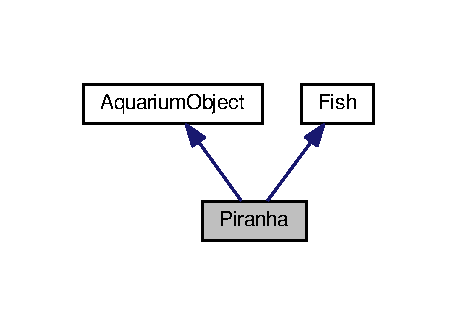
\includegraphics[width=220pt]{class_piranha__inherit__graph}
\end{center}
\end{figure}


Collaboration diagram for Piranha\+:
\nopagebreak
\begin{figure}[H]
\begin{center}
\leavevmode
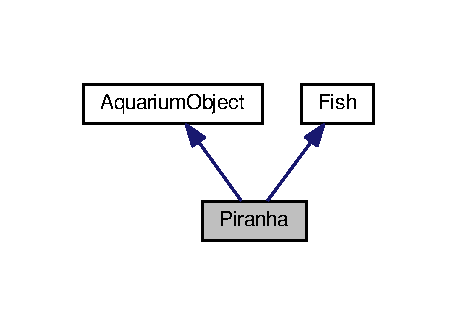
\includegraphics[width=220pt]{class_piranha__coll__graph}
\end{center}
\end{figure}
\subsection*{Public Member Functions}
\begin{DoxyCompactItemize}
\item 
void \mbox{\hyperlink{class_piranha_ac9bde9a286096cf199bdb1df5434a8c8}{eat}} ()
\item 
void \mbox{\hyperlink{class_piranha_ac7d4af6cc29513e5bd351cbbaf25cc0b}{drop\+Coin}} ()
\item 
void \mbox{\hyperlink{class_piranha_a65ebc6270eb3b1eeaad1c9c0eb53d399}{move}} (final Graphics g)
\end{DoxyCompactItemize}


\subsection{Detailed Description}
Class \mbox{\hyperlink{class_piranha}{Piranha}}. This class implements \mbox{\hyperlink{interface_fish}{Fish}}. \mbox{\hyperlink{class_piranha}{Piranha}} is an aquarium object than can be bought during the game using the coins that the player has. It also can drop coin directly after \mbox{\hyperlink{class_piranha}{Piranha}} eats \mbox{\hyperlink{class_guppy}{Guppy}}. 

\subsection{Member Function Documentation}
\mbox{\Hypertarget{class_piranha_ac7d4af6cc29513e5bd351cbbaf25cc0b}\label{class_piranha_ac7d4af6cc29513e5bd351cbbaf25cc0b}} 
\index{Piranha@{Piranha}!drop\+Coin@{drop\+Coin}}
\index{drop\+Coin@{drop\+Coin}!Piranha@{Piranha}}
\subsubsection{\texorpdfstring{drop\+Coin()}{dropCoin()}}
{\footnotesize\ttfamily void Piranha.\+drop\+Coin (\begin{DoxyParamCaption}{ }\end{DoxyParamCaption})\hspace{0.3cm}{\ttfamily [inline]}}

This method will drop coin. \mbox{\hyperlink{class_piranha}{Piranha}} will drop coin directly after eating. Also, coin value vary and be calculated as follows\+: G\+U\+P\+P\+Y\+\_\+\+P\+R\+I\+CE multiply by S\+T\+A\+T\+E\+\_\+\+O\+F\+\_\+\+G\+U\+P\+PY added by one. 

Implements \mbox{\hyperlink{interface_fish_ad37facd4d5859411cf433520f03ae0b8}{Fish}}.

\mbox{\Hypertarget{class_piranha_ac9bde9a286096cf199bdb1df5434a8c8}\label{class_piranha_ac9bde9a286096cf199bdb1df5434a8c8}} 
\index{Piranha@{Piranha}!eat@{eat}}
\index{eat@{eat}!Piranha@{Piranha}}
\subsubsection{\texorpdfstring{eat()}{eat()}}
{\footnotesize\ttfamily void Piranha.\+eat (\begin{DoxyParamCaption}{ }\end{DoxyParamCaption})\hspace{0.3cm}{\ttfamily [inline]}}

This method will eat \mbox{\hyperlink{class_guppy}{Guppy}}. \mbox{\hyperlink{class_piranha}{Piranha}} only eats when \mbox{\hyperlink{class_piranha}{Piranha}} is hungry and will try to reach the nearest food available. 

Implements \mbox{\hyperlink{interface_fish_a72d533bdc4ac39f4ffd93d70504efed8}{Fish}}.

\mbox{\Hypertarget{class_piranha_a65ebc6270eb3b1eeaad1c9c0eb53d399}\label{class_piranha_a65ebc6270eb3b1eeaad1c9c0eb53d399}} 
\index{Piranha@{Piranha}!move@{move}}
\index{move@{move}!Piranha@{Piranha}}
\subsubsection{\texorpdfstring{move()}{move()}}
{\footnotesize\ttfamily void Piranha.\+move (\begin{DoxyParamCaption}\item[{final Graphics}]{g }\end{DoxyParamCaption})\hspace{0.3cm}{\ttfamily [inline]}}

This method is used to move the object. \mbox{\hyperlink{class_piranha}{Piranha}}\textquotesingle{}s movements are described as below\+:
\begin{DoxyEnumerate}
\item If \mbox{\hyperlink{class_piranha}{Piranha}} is not hungry, \mbox{\hyperlink{class_piranha}{Piranha}} will move randomly.
\item If \mbox{\hyperlink{class_piranha}{Piranha}} is hungry and there is no food available, then it moves randomly.
\item If \mbox{\hyperlink{class_piranha}{Piranha}} is hungry and there is food available, then it moves towards the nearest food.
\end{DoxyEnumerate}


\begin{DoxyParams}{Parameters}
{\em g} & is Graphics \\
\hline
\end{DoxyParams}


The documentation for this class was generated from the following file\+:\begin{DoxyCompactItemize}
\item 
/media/malfianrasyidin/\+A\+L\+F\+I\+A\+N/java/\+Arkav\+Quarium\+Java/src/Piranha.\+java\end{DoxyCompactItemize}

\hypertarget{class_snail}{}\section{Snail Class Reference}
\label{class_snail}\index{Snail@{Snail}}


Inheritance diagram for Snail\+:
\nopagebreak
\begin{figure}[H]
\begin{center}
\leavevmode
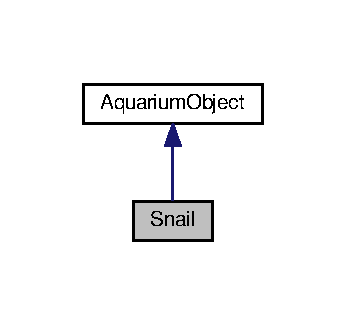
\includegraphics[width=166pt]{class_snail__inherit__graph}
\end{center}
\end{figure}


Collaboration diagram for Snail\+:
\nopagebreak
\begin{figure}[H]
\begin{center}
\leavevmode
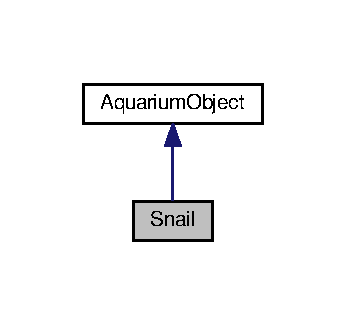
\includegraphics[width=166pt]{class_snail__coll__graph}
\end{center}
\end{figure}
\subsection*{Public Member Functions}
\begin{DoxyCompactItemize}
\item 
void \mbox{\hyperlink{class_snail_a99cf307667441615ed79de2fd4ba5fe5}{set\+Money}} (final \mbox{\hyperlink{class_node}{Node}}$<$ Integer $>$ p\+Money)
\item 
double \mbox{\hyperlink{class_snail_a6b26b21e7bf3702c9e263cae1a9bc3ad}{get\+Radius}} ()
\item 
\mbox{\hyperlink{class_node}{Node}}$<$ Integer $>$ \mbox{\hyperlink{class_snail_ad57c8cb98f65b980483ce326bc7e6031}{get\+Money}} ()
\item 
void \mbox{\hyperlink{class_snail_ad077a58207472113fae8ec37696d83e3}{grab\+Coin}} (final \mbox{\hyperlink{class_coin}{Coin}} coin)
\item 
void \mbox{\hyperlink{class_snail_a88ef832abb1c54f196242d47431ff866}{move}} (final Graphics g)
\end{DoxyCompactItemize}
\subsection*{Static Public Member Functions}
\begin{DoxyCompactItemize}
\item 
static void \mbox{\hyperlink{class_snail_a0c21e4603e41e352e2d3d91d172e0b9e}{set\+List\+Coin}} (final \mbox{\hyperlink{class_linked_list}{Linked\+List}}$<$ \mbox{\hyperlink{class_coin}{Coin}} $>$ p\+List\+Coin)
\item 
static void \mbox{\hyperlink{class_snail_a90cd994cbdd5daae66bade7702472dac}{set\+Snail\+Left}} (final Buffered\+Image p\+Snail\+Left)
\item 
static void \mbox{\hyperlink{class_snail_a604a57abe628e6f708d61365630fdc9e}{set\+Snail\+Right}} (final Buffered\+Image p\+Snail\+Right)
\item 
static \mbox{\hyperlink{class_linked_list}{Linked\+List}}$<$ \mbox{\hyperlink{class_coin}{Coin}} $>$ \mbox{\hyperlink{class_snail_ae777445d6e995a27c4049fbf9a51c7a5}{get\+List\+Coin}} ()
\end{DoxyCompactItemize}


\subsection{Detailed Description}
Class \mbox{\hyperlink{class_snail}{Snail}}. This class is derived from \mbox{\hyperlink{class_aquarium_object}{Aquarium\+Object}}. \mbox{\hyperlink{class_snail}{Snail}} is an aquarium object that collects coin. 

\subsection{Member Function Documentation}
\mbox{\Hypertarget{class_snail_ae777445d6e995a27c4049fbf9a51c7a5}\label{class_snail_ae777445d6e995a27c4049fbf9a51c7a5}} 
\index{Snail@{Snail}!get\+List\+Coin@{get\+List\+Coin}}
\index{get\+List\+Coin@{get\+List\+Coin}!Snail@{Snail}}
\subsubsection{\texorpdfstring{get\+List\+Coin()}{getListCoin()}}
{\footnotesize\ttfamily static \mbox{\hyperlink{class_linked_list}{Linked\+List}}$<$\mbox{\hyperlink{class_coin}{Coin}}$>$ Snail.\+get\+List\+Coin (\begin{DoxyParamCaption}{ }\end{DoxyParamCaption})\hspace{0.3cm}{\ttfamily [inline]}, {\ttfamily [static]}}

Get list of coin.

\begin{DoxyReturn}{Returns}
list of coin 
\end{DoxyReturn}
\mbox{\Hypertarget{class_snail_ad57c8cb98f65b980483ce326bc7e6031}\label{class_snail_ad57c8cb98f65b980483ce326bc7e6031}} 
\index{Snail@{Snail}!get\+Money@{get\+Money}}
\index{get\+Money@{get\+Money}!Snail@{Snail}}
\subsubsection{\texorpdfstring{get\+Money()}{getMoney()}}
{\footnotesize\ttfamily \mbox{\hyperlink{class_node}{Node}}$<$Integer$>$ Snail.\+get\+Money (\begin{DoxyParamCaption}{ }\end{DoxyParamCaption})\hspace{0.3cm}{\ttfamily [inline]}}

Get money.

\begin{DoxyReturn}{Returns}
node of money 
\end{DoxyReturn}
\mbox{\Hypertarget{class_snail_a6b26b21e7bf3702c9e263cae1a9bc3ad}\label{class_snail_a6b26b21e7bf3702c9e263cae1a9bc3ad}} 
\index{Snail@{Snail}!get\+Radius@{get\+Radius}}
\index{get\+Radius@{get\+Radius}!Snail@{Snail}}
\subsubsection{\texorpdfstring{get\+Radius()}{getRadius()}}
{\footnotesize\ttfamily double Snail.\+get\+Radius (\begin{DoxyParamCaption}{ }\end{DoxyParamCaption})\hspace{0.3cm}{\ttfamily [inline]}}

Get snail radius.

\begin{DoxyReturn}{Returns}
snail radius 
\end{DoxyReturn}
\mbox{\Hypertarget{class_snail_ad077a58207472113fae8ec37696d83e3}\label{class_snail_ad077a58207472113fae8ec37696d83e3}} 
\index{Snail@{Snail}!grab\+Coin@{grab\+Coin}}
\index{grab\+Coin@{grab\+Coin}!Snail@{Snail}}
\subsubsection{\texorpdfstring{grab\+Coin()}{grabCoin()}}
{\footnotesize\ttfamily void Snail.\+grab\+Coin (\begin{DoxyParamCaption}\item[{final \mbox{\hyperlink{class_coin}{Coin}}}]{coin }\end{DoxyParamCaption})\hspace{0.3cm}{\ttfamily [inline]}}

This method is used to grab the coin.


\begin{DoxyParams}{Parameters}
{\em coin} & is the coin \\
\hline
\end{DoxyParams}
\mbox{\Hypertarget{class_snail_a88ef832abb1c54f196242d47431ff866}\label{class_snail_a88ef832abb1c54f196242d47431ff866}} 
\index{Snail@{Snail}!move@{move}}
\index{move@{move}!Snail@{Snail}}
\subsubsection{\texorpdfstring{move()}{move()}}
{\footnotesize\ttfamily void Snail.\+move (\begin{DoxyParamCaption}\item[{final Graphics}]{g }\end{DoxyParamCaption})\hspace{0.3cm}{\ttfamily [inline]}}

This method is used to move the object. \mbox{\hyperlink{class_snail}{Snail}}\textquotesingle{}s movements are described as below\+:
\begin{DoxyEnumerate}
\item If there is coin available, \mbox{\hyperlink{class_snail}{Snail}} will move towards the nearest coin.
\item If there is no coin available, \mbox{\hyperlink{class_snail}{Snail}} will just stay at its current location.
\end{DoxyEnumerate}


\begin{DoxyParams}{Parameters}
{\em g} & is Graphics \\
\hline
\end{DoxyParams}
\mbox{\Hypertarget{class_snail_a0c21e4603e41e352e2d3d91d172e0b9e}\label{class_snail_a0c21e4603e41e352e2d3d91d172e0b9e}} 
\index{Snail@{Snail}!set\+List\+Coin@{set\+List\+Coin}}
\index{set\+List\+Coin@{set\+List\+Coin}!Snail@{Snail}}
\subsubsection{\texorpdfstring{set\+List\+Coin()}{setListCoin()}}
{\footnotesize\ttfamily static void Snail.\+set\+List\+Coin (\begin{DoxyParamCaption}\item[{final \mbox{\hyperlink{class_linked_list}{Linked\+List}}$<$ \mbox{\hyperlink{class_coin}{Coin}} $>$}]{p\+List\+Coin }\end{DoxyParamCaption})\hspace{0.3cm}{\ttfamily [inline]}, {\ttfamily [static]}}

Set list of coin.


\begin{DoxyParams}{Parameters}
{\em p\+List\+Coin} & is list of coin \\
\hline
\end{DoxyParams}
\mbox{\Hypertarget{class_snail_a99cf307667441615ed79de2fd4ba5fe5}\label{class_snail_a99cf307667441615ed79de2fd4ba5fe5}} 
\index{Snail@{Snail}!set\+Money@{set\+Money}}
\index{set\+Money@{set\+Money}!Snail@{Snail}}
\subsubsection{\texorpdfstring{set\+Money()}{setMoney()}}
{\footnotesize\ttfamily void Snail.\+set\+Money (\begin{DoxyParamCaption}\item[{final \mbox{\hyperlink{class_node}{Node}}$<$ Integer $>$}]{p\+Money }\end{DoxyParamCaption})\hspace{0.3cm}{\ttfamily [inline]}}

Set money.


\begin{DoxyParams}{Parameters}
{\em p\+Money} & is money \\
\hline
\end{DoxyParams}
\mbox{\Hypertarget{class_snail_a90cd994cbdd5daae66bade7702472dac}\label{class_snail_a90cd994cbdd5daae66bade7702472dac}} 
\index{Snail@{Snail}!set\+Snail\+Left@{set\+Snail\+Left}}
\index{set\+Snail\+Left@{set\+Snail\+Left}!Snail@{Snail}}
\subsubsection{\texorpdfstring{set\+Snail\+Left()}{setSnailLeft()}}
{\footnotesize\ttfamily static void Snail.\+set\+Snail\+Left (\begin{DoxyParamCaption}\item[{final Buffered\+Image}]{p\+Snail\+Left }\end{DoxyParamCaption})\hspace{0.3cm}{\ttfamily [inline]}, {\ttfamily [static]}}

Set image of \mbox{\hyperlink{class_snail}{Snail}} facing left.


\begin{DoxyParams}{Parameters}
{\em p\+Snail\+Left} & is Buffered\+Image \\
\hline
\end{DoxyParams}
\mbox{\Hypertarget{class_snail_a604a57abe628e6f708d61365630fdc9e}\label{class_snail_a604a57abe628e6f708d61365630fdc9e}} 
\index{Snail@{Snail}!set\+Snail\+Right@{set\+Snail\+Right}}
\index{set\+Snail\+Right@{set\+Snail\+Right}!Snail@{Snail}}
\subsubsection{\texorpdfstring{set\+Snail\+Right()}{setSnailRight()}}
{\footnotesize\ttfamily static void Snail.\+set\+Snail\+Right (\begin{DoxyParamCaption}\item[{final Buffered\+Image}]{p\+Snail\+Right }\end{DoxyParamCaption})\hspace{0.3cm}{\ttfamily [inline]}, {\ttfamily [static]}}

Set image of \mbox{\hyperlink{class_snail}{Snail}} facing right.


\begin{DoxyParams}{Parameters}
{\em p\+Snail\+Right} & is Buffered\+Image \\
\hline
\end{DoxyParams}


The documentation for this class was generated from the following file\+:\begin{DoxyCompactItemize}
\item 
/media/malfianrasyidin/\+A\+L\+F\+I\+A\+N/java/\+Arkav\+Quarium\+Java/src/Snail.\+java\end{DoxyCompactItemize}

%--- End generated contents ---

% Index
\backmatter
\newpage
\phantomsection
\clearemptydoublepage
\addcontentsline{toc}{chapter}{Index}
\printindex

\end{document}
